% EN3150 Assignment 03 - Resource-Constrained CNN for Edge Image Classification
%
% Build from the repository root with one command:
%
%     python scripts/build_report.py
%
% Ported from the group's EN3150 A02 template (issue #23): same page geometry,
% packages, code listing styles, footer and title-page layout.
%
% Each task section's prose lives in report/sections/*.tex, owned by the issue
% named beside its \input. Every number reaches this document through a
% generated file in tables/ or figures/ - never hand-typed. A generated file
% that does not exist yet renders as a visible "Pending" box (see
% \generatedtable and \generatedfigure below) instead of breaking the build.

\documentclass[11pt]{article}

\usepackage[a4paper,margin=1in]{geometry}
\usepackage{amsmath,amssymb}
\usepackage{graphicx}
\usepackage{xcolor}
\usepackage{listings}
\usepackage{hyperref}
\usepackage{booktabs}
\usepackage{float}
\usepackage{enumitem}
\usepackage{fancyhdr}

% ---------------------------------------------------------------- listings --
% Code styles carried over unchanged from A02.

\definecolor{codebg}{RGB}{234,243,224}
\definecolor{codegreen}{RGB}{0,128,0}
\definecolor{codeblue}{RGB}{0,0,180}
\definecolor{codegray}{RGB}{110,110,110}
\definecolor{codeorange}{RGB}{180,90,0}

\lstdefinestyle{python}{
    backgroundcolor=\color{codebg},
    basicstyle=\ttfamily\footnotesize,
    keywordstyle=\color{codeblue}\bfseries,
    commentstyle=\color{codegray}\itshape,
    stringstyle=\color{codeorange},
    numbers=none,
    breaklines=true,
    breakatwhitespace=false,
    showstringspaces=false,
    frame=single,
    framerule=0pt,
    xleftmargin=2pt,
    xrightmargin=2pt,
    tabsize=4,
    language=Python,
    columns=fullflexible,
    aboveskip=8pt,
    belowskip=8pt
}

\lstdefinestyle{output}{
    backgroundcolor=\color{white},
    basicstyle=\ttfamily\footnotesize,
    frame=single,
    framerule=0.4pt,
    rulecolor=\color{black!40},
    breaklines=true,
    xleftmargin=2pt,
    xrightmargin=2pt,
    aboveskip=4pt,
    belowskip=8pt
}

\lstset{style=python}

\hypersetup{
    colorlinks=true,
    linkcolor=red!70!black,
    urlcolor=blue,
    citecolor=red!70!black
}

\pagestyle{fancy}
\fancyhf{}
\fancyfoot[C]{\thepage}
\renewcommand{\headrulewidth}{0pt}

% ------------------------------------------------------ skeleton helpers --

% Red, bracketed text for anything a human must still fill in. Red so that a
% placeholder left in by accident is impossible to miss in the final PDF;
% #26 (final assembly) must leave none.
\newcommand{\placeholder}[1]{\textcolor{red}{\textbf{[#1]}}}

% A framed note for content an open issue will supply.
\newcommand{\pending}[1]{%
  \begin{center}
  \fbox{\parbox{0.9\linewidth}{\centering\itshape\color{red!70!black}Pending: #1}}%
  \end{center}}

% Generated artifacts that may not exist yet. Each takes the path the
% generator writes to and the issue that produces it. Once the file exists it
% is used as-is; until then the PDF shows where it will go and who owes it.
%   \generatedtable{tables/x.tex}{\#22}
%   \generatedfigure[width=0.8\linewidth]{figures/x.png}{\#22}
% \detokenize prints the path verbatim: generated file names contain
% underscores, which LaTeX would otherwise read as math subscripts.
\newcommand{\generatedtable}[2]{%
  \IfFileExists{#1}{\input{#1}}%
    {\pending{generated table \texttt{\detokenize{#1}} (#2)}}}
\newcommand{\generatedfigure}[3][width=\linewidth]{%
  \IfFileExists{#2}{\includegraphics[#1]{#2}}%
    {\pending{generated figure \texttt{\detokenize{#2}} (#3)}}}

% ------------------------------------------------------------ title data --
% Filled in by #26 (final assembly). The submission file name is
% <groupno>_A03_EN3150.

\newcommand{\groupno}{9}
\newcommand{\repourl}{https://github.com/dpiyumal2319/pattern-recognition-cnn-edge}
% The build date: the submitted PDF is built on submission day.
\newcommand{\submissiondate}{\today}

\title{}
\date{}

\begin{document}

% ------------------------------------------------------------- title page --
\begin{titlepage}
\centering
\vspace*{1.5cm}
{\bfseries Department of Electronic \& Telecommunication Engineering, University of\\
Moratuwa, Sri Lanka.\par}

\vspace{1.5cm}

\includegraphics[width=0.18\textwidth]{figures/uom_logo.png}

\vspace{1.5cm}
{\LARGE\bfseries Resource-Constrained CNN for\\ Edge Image Classification\par}
\vspace{0.4cm}
{\large EN3150 Assignment 03\par}

\vspace{1.5cm}
{\large\bfseries Group \groupno\par}
\vspace{0.6cm}
{\large
\begin{tabular}{l@{\quad--\quad}l}
  WIJETHUNGA W. M. D. P & 220727G \\
  WIJERATNE E.N.K & 220717C \\
  GALLAGE A.H. & 220172A \\
  DISANAYAKA J.R.S. & 220132D \\
\end{tabular}\par}

\vspace{1.5cm}
{\bfseries EN3150 -- Pattern Recognition\par}
Submitted in partial fulfillment of the requirements for the module

\vspace{0.8cm}
{\bfseries Code repository\par}
\url{\repourl}

\vfill

{\bfseries Date\par}
\submissiondate

\end{titlepage}

% --------------------------------------------------------------- contents --
\tableofcontents
\vspace{1cm}

\noindent All code, configurations and result files are in the group's
repository at \url{\repourl}. No result in this report is typed by hand: every
table and figure is generated from the committed result files by the
repository's \texttt{build\_tables.py} and \texttt{build\_figures.py} scripts.

\newpage

% =========================================================================
\section{Task 1: Data Preparation}
\label{sec:task1}

% Owned by #24 (dataset and methodology). The split table is generated from
% data/splits.csv by scripts/build_tables.py --table dataset.

\subsection{Dataset}
\label{sec:dataset}

We use EuroSAT~\cite{helber2019eurosat}, a land-use and land-cover dataset
containing 27,000 labelled, geo-referenced Sentinel-2 image patches across ten
classes: AnnualCrop, Forest, HerbaceousVegetation, Highway, Industrial,
Pasture, PermanentCrop, Residential, River, and SeaLake. Although the original
dataset includes all 13 Sentinel-2 spectral bands, this work uses the RGB
version, which contains the three visible bands stored as 8-bit images. The
dataset is available under the MIT licence and was downloaded through
\texttt{torchvision}~\cite{torchvision2016} version 0.20 or later, which uses
the maintained Hugging Face mirror. Because each class represents a land-cover
category viewed from an overhead perspective, orientation changes such as
flips and 90-degree rotations do not alter the class label, which supports the
augmentation choices described in Section~\ref{sec:data-preparation}.

\paragraph{Input resolution.}
All EuroSAT images have a native resolution of $64\times64$ pixels. Since the
assignment specifies a maximum input resolution of $64\times64$ for the
low-resource setting, the dataset already satisfies this requirement and no
downscaling is needed. The custom models therefore use the original images
directly, without reducing their spatial resolution.
Figure~\ref{fig:data-augmentation-grid} shows one native sample from each
class. The only resizing beyond the native resolution is an upsampling step to
$224\times224$ for the supplementary SOTA resolution experiment in Task~5,
where the pretrained models are also evaluated at their standard design
resolution.

\paragraph{Split.}
The dataset was divided once into training, validation, and test sets using
the required 70/15/15 proportions. The split was stratified by class, so each
class was divided independently and the class distribution remains consistent
across all three sets. Class sizes range from 2,000 to 3,000 images
(Table~\ref{tab:dataset-split}), and these sizes allow the 70/15/15
proportions to be applied exactly. Within each class, image files were sorted
by name and then shuffled using a fixed seed of 42. This makes the split
reproducible and ensures that the same partition is obtained across different
machines.

\paragraph{One partition for every experiment.}
The train, validation, and test assignment for each image is recorded in the
committed manifest, \texttt{data/splits.csv}. All experiments use this same
file, including the custom models, optimizer comparison, and fine-tuned SOTA
models, rather than generating new splits. This keeps the data partition fixed
across experiments and satisfies the requirement that the SOTA models use the
same splits as the custom networks. Table~\ref{tab:dataset-split} is generated
directly from this manifest. The validation set is used for model and
optimizer selection, while the test set is reserved for final evaluation after
training.

\begin{table}[htbp]
  \centering
  \caption{Images per class in each set, generated from the committed split
  manifest \texttt{data/splits.csv}.}
  \label{tab:dataset-split}
  \generatedtable{tables/dataset.tex}{\#24}
\end{table}
            % #24: source, classes, split table
% Preprocessing implemented by #3; methodology write-up by #24.

\subsection{Preprocessing and augmentation}
\label{sec:data-preparation}

\paragraph{Standardisation.}
Each RGB channel is standardised,
\begin{equation}
  x' = \frac{x - \mu_c}{\sigma_c},
  \label{eq:standardisation}
\end{equation}
giving zero-mean, unit-variance feature scaling. Pixels are first scaled to
$[0,1]$; $\mu_c$ and $\sigma_c$ are the
per-channel mean and population standard deviation. Without this step the
three channels enter the first convolution with different offsets and spreads,
so the gradient scale differs per channel and a single learning rate suits none
of them well. The same pipeline, with the same EuroSAT statistics, feeds the
pretrained models in Task~5. Those networks were trained on standardised
inputs, but with the channel statistics of ImageNet~\cite{deng2009imagenet};
we use EuroSAT's own instead,
so that every model in the comparison sees identically preprocessed images and
the standardisation reflects the satellite data actually being classified.

\paragraph{Statistics from the training set only.}
Estimating preprocessing statistics before splitting would leak information:
if $\mu_c$ and $\sigma_c$ were computed over all
27,000 images, the preprocessing applied to the test set would already reflect
the test images, and the test score would no longer be a fair estimate of
performance on unseen data. We therefore fix the split first and estimate
$\mu_c$ and $\sigma_c$ from the training set alone (Table~\ref{tab:dataset-split}) --- before any
augmentation, at native resolution --- then apply those same values unchanged to
the validation and test sets, as an unseen deployment image would be treated.
The statistics are computed once and cached, so every experiment normalises
identically.

\paragraph{Augmentation.}
Augmentation artificially expands the size and diversity of a dataset through
transformations such as rotation and flipping. During training only, each image independently receives a horizontal
flip and a vertical flip, each with probability 0.5, and a rotation by a
uniformly chosen multiple of $90^\circ$. Together these produce all eight
orientations of the square image, freshly sampled every epoch
(Figure~\ref{fig:data-augmentation-grid}).

These transformations are \emph{label-preserving} for EuroSAT specifically. The
images are taken from directly overhead, so ``up'' in the image has no physical
meaning: a river, a highway or a field is the same land-cover class whichever
way it is rotated or mirrored. The same would not hold for ground-level
photographs, where a vertically flipped scene is not a realistic image. The
$90^\circ$ multiples are also exact pixel permutations of a square grid, so no
interpolation blurs the image and no corner is filled with padding.

Other common augmentations were deliberately not used. Random crops and
rescaling would change the apparent size of objects, but Sentinel-2 imagery has
a fixed ground resolution, so object size is real evidence --- a residential
block and an industrial site differ partly in scale --- and at $64\times64$ a
crop also discards much of a small image. Colour jitter was rejected because
colour carries the class: water, vegetation and bare soil differ chiefly in
their spectral response, so altering hue could turn one class's appearance into
another's.

\paragraph{Evaluation preprocessing and class balance.}
Validation and test images are only converted to tensors and standardised with
the training statistics, so every evaluation is deterministic. The classes are
mildly imbalanced (2,000 to 3,000 images; Table~\ref{tab:dataset-split}).
Under-sampling and synthetic minority samples are possible remedies, but at a
ratio of 1.5:1 neither was needed: stratification
keeps the imbalance identical across the three sets, and the evaluation reports
macro-averaged precision and recall alongside accuracy, so the smaller classes
are not hidden by the larger ones.

\begin{figure}[htbp]
    \centering
    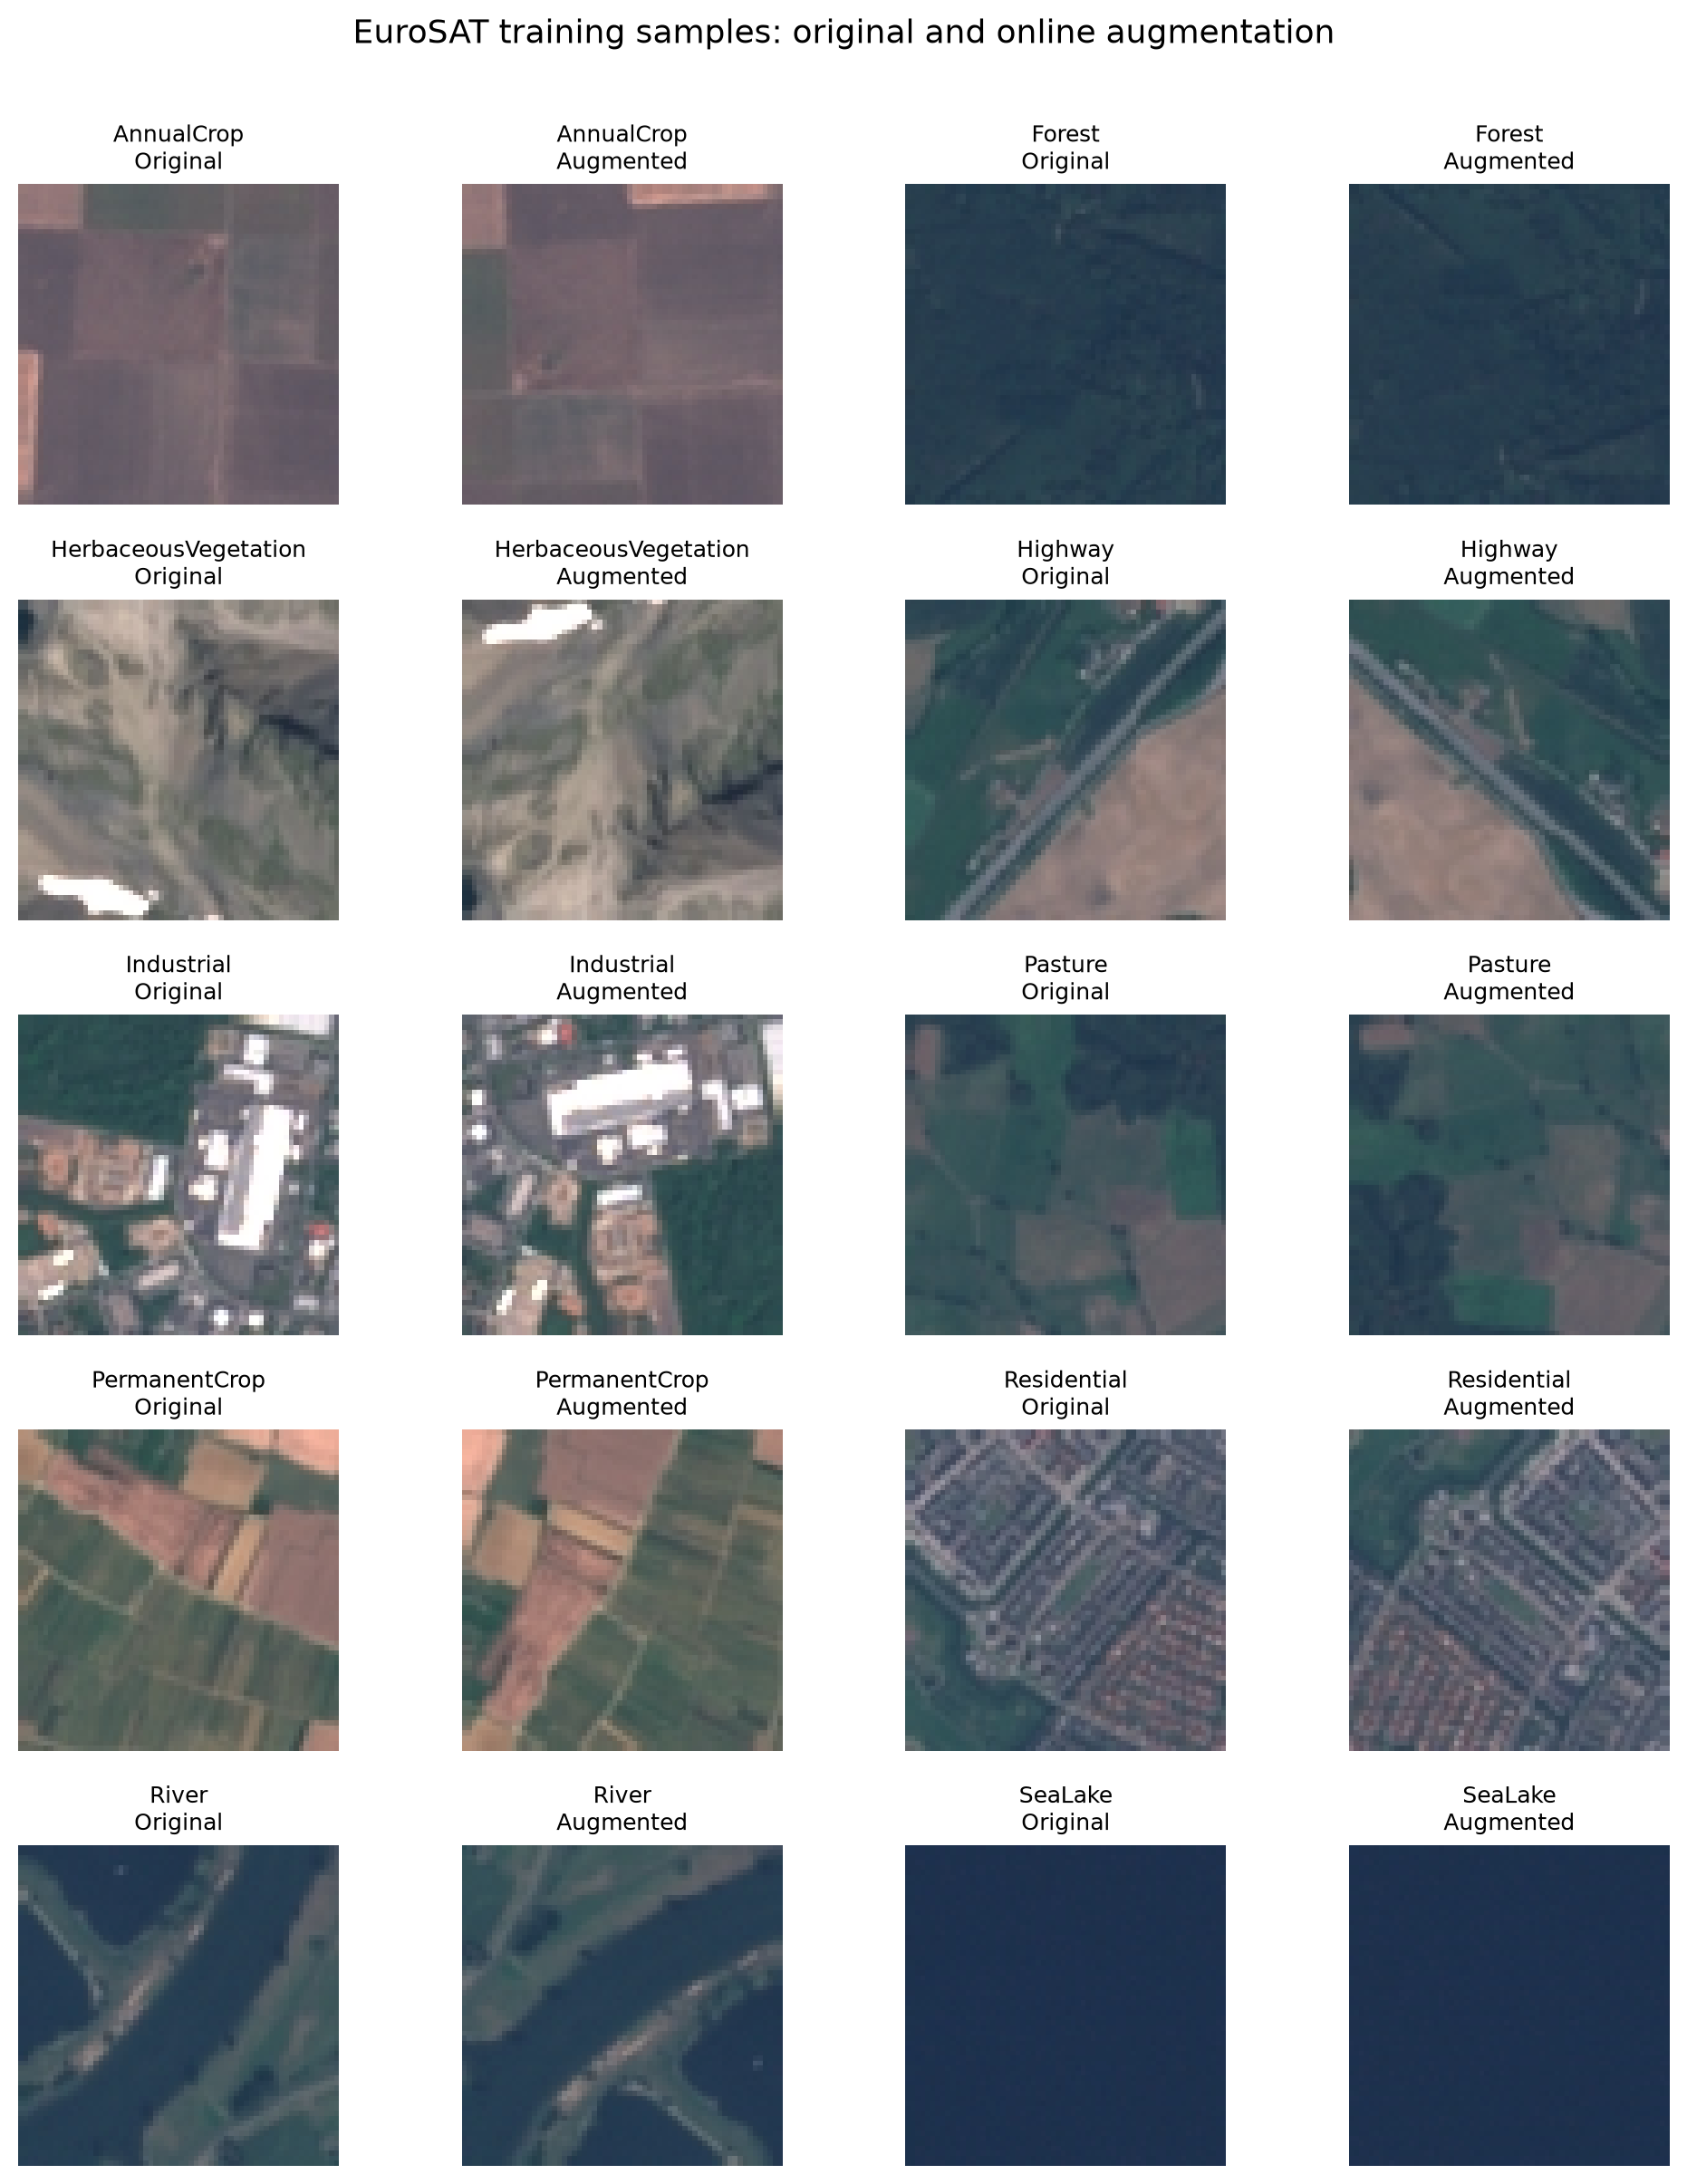
\includegraphics[width=\textwidth]{figures/data_augmentation_grid.png}
    \caption{One training image from each EuroSAT class before and after the
    configured online augmentation. EuroSAT images are natively
    $64\times64$ pixels, so these are shown at their original resolution.}
    \label{fig:data-augmentation-grid}
\end{figure}
   % #3:  normalisation, augmentation, sample grid

% =========================================================================
\section{Task 2: Custom Architecture Design}
\label{sec:task2}

\subsection{Custom architecture design}
\label{sec:custom-architecture}

Both custom networks take a $64\times64$ RGB image and output ten class
logits.  Each feature-extraction stage has a valid $3\times3$ convolutional
operation with stride~1 and no padding, followed by ReLU and $2\times2$ max
pooling with stride~2.  Because of this, the spatial size goes through
$64\rightarrow62\rightarrow31\rightarrow29\rightarrow14\rightarrow12
\rightarrow6$ over the three stages.  Both networks use channel widths of 32,
64 and 128 and hidden fully connected widths of 128 and 64.  The only
differences are that Model B replaces Model A's standard convolutions with
depthwise separable convolutions, and replaces its flattened head with global
average pooling (GAP).

All convolutional and dense layers have biases, and there is no batch
normalisation in either model.  During training, dropout with probability 0.2
is applied right before each hidden dense layer, and it is turned off for
validation and inference.  The final dense layer outputs raw logits, so there
is no ReLU or softmax after it.

A standard convolution has
\begin{equation}
  P_{\mathrm{conv}}=(K_hK_wC_{\mathrm{in}}+1)C_{\mathrm{out}},
\end{equation}
where the added one is the bias of each output channel.  A depthwise and
pointwise pair instead has
\begin{equation}
  P_{\mathrm{sep}}=(K_hK_w+1)C_{\mathrm{in}}
  +(C_{\mathrm{in}}+1)C_{\mathrm{out}}.
\end{equation}
A dense layer has $(N_{\mathrm{in}}+1)N_{\mathrm{out}}$ parameters.  For one
image, we count convolution MACs as
$K_hK_wC_{\mathrm{in}}C_{\mathrm{out}}H_{\mathrm{out}}W_{\mathrm{out}}$
and dense MACs as $N_{\mathrm{in}}N_{\mathrm{out}}$, and bias additions are
not counted.  Max pooling, ReLU, dropout, flatten and GAP have no trainable
parameters.  Pooling and averaging operations are also left out of the MAC
total, because the project profiler does not count them and the hand
derivation should match the profiler exactly.

\subsubsection{Model A: standard CNN}

Model A flattens the final feature map into $128\times6\times6=4{,}608$
values before the first dense layer, and
Table~\ref{tab:model-a-hand-derivation} derives the parameters and MACs of
every layer from these shapes.

\begin{table}[htbp]
  \centering
  \caption{Hand-derived parameters and MACs for Model A.}
  \label{tab:model-a-hand-derivation}
  \resizebox{\linewidth}{!}{%
  \begin{tabular}{llll}
    \hline
    Layer & Output & Parameter arithmetic & MAC arithmetic \\
    \hline
    Conv 1 & $32\times62\times62$ & $(3\times3\times3+1)\times32=896$
      & $3\times3\times3\times32\times62^2=3{,}321{,}216$ \\
    MaxPool 1 & $32\times31\times31$ & $0$ & $0$ (not profiled) \\
    Conv 2 & $64\times29\times29$ & $(3\times3\times32+1)\times64=18{,}496$
      & $3\times3\times32\times64\times29^2=15{,}501{,}312$ \\
    MaxPool 2 & $64\times14\times14$ & $0$ & $0$ (not profiled) \\
    Conv 3 & $128\times12\times12$ & $(3\times3\times64+1)\times128=73{,}856$
      & $3\times3\times64\times128\times12^2=10{,}616{,}832$ \\
    MaxPool 3 & $128\times6\times6$ & $0$ & $0$ (not profiled) \\
    Flatten & $4{,}608$ & $0$ & $0$ \\
    Dense 1 & $128$ & $(4{,}608+1)\times128=589{,}952$
      & $4{,}608\times128=589{,}824$ \\
    Dense 2 & $64$ & $(128+1)\times64=8{,}256$
      & $128\times64=8{,}192$ \\
    Output & $10$ & $(64+1)\times10=650$ & $64\times10=640$ \\
    \hline
    Total & & $692{,}106$ & $30{,}038{,}016$ \\
    \hline
  \end{tabular}%
  }
\end{table}

The convolutional stack has only $93{,}248$ parameters, while the dense head
has $598{,}858$, which is $86.5\%$ of the total.  So the head is the part that
Model B has to cut if it is to meet its parameter budget.

\subsubsection{Model B: depthwise separable CNN}

In each Model B stage, the depthwise step applies one $3\times3$ filter to
each input channel, and the pointwise $1\times1$ step then mixes those
channels.  There is only one ReLU per stage, and it comes after the pointwise
step.  Table~\ref{tab:model-b-hand-derivation} lists the two convolutions as
separate rows so that the cost of each step can be seen.

\begin{table}[htbp]
  \centering
  \caption{Hand-derived parameters and MACs for Model B. DW and PW denote
  depthwise $3\times3$ and pointwise $1\times1$ convolution.}
  \label{tab:model-b-hand-derivation}
  \resizebox{\linewidth}{!}{%
  \begin{tabular}{llll}
    \hline
    Layer & Output & Parameter arithmetic & MAC arithmetic \\
    \hline
    DW 1 & $3\times62\times62$ & $(3\times3+1)\times3=30$
      & $3\times3\times3\times62^2=103{,}788$ \\
    PW 1 & $32\times62\times62$ & $(3+1)\times32=128$
      & $3\times32\times62^2=369{,}024$ \\
    MaxPool 1 & $32\times31\times31$ & $0$ & $0$ (not profiled) \\
    DW 2 & $32\times29\times29$ & $(3\times3+1)\times32=320$
      & $3\times3\times32\times29^2=242{,}208$ \\
    PW 2 & $64\times29\times29$ & $(32+1)\times64=2{,}112$
      & $32\times64\times29^2=1{,}722{,}368$ \\
    MaxPool 2 & $64\times14\times14$ & $0$ & $0$ (not profiled) \\
    DW 3 & $64\times12\times12$ & $(3\times3+1)\times64=640$
      & $3\times3\times64\times12^2=82{,}944$ \\
    PW 3 & $128\times12\times12$ & $(64+1)\times128=8{,}320$
      & $64\times128\times12^2=1{,}179{,}648$ \\
    MaxPool 3 & $128\times6\times6$ & $0$ & $0$ (not profiled) \\
    GAP and flatten & $128$ & $0$ & $0$ (not profiled) \\
    Dense 1 & $128$ & $(128+1)\times128=16{,}512$
      & $128\times128=16{,}384$ \\
    Dense 2 & $64$ & $(128+1)\times64=8{,}256$
      & $128\times64=8{,}192$ \\
    Output & $10$ & $(64+1)\times10=650$ & $64\times10=640$ \\
    \hline
    Total & & $36{,}968$ & $3{,}725{,}196$ \\
    \hline
  \end{tabular}%
  }
\end{table}

GAP reduces the $128\times6\times6$ tensor to 128 channel means before the
dense stack, so Model B does not need the $4{,}608\rightarrow128$ layer that
dominates Model A.

The separable blocks have $11{,}550$ parameters and the GAP-based dense head
has $25{,}418$, which puts Model B $63{,}032$ parameters below the
100,000-parameter limit.  Keeping a flattened head would leave a
$589{,}952$-parameter first dense layer, and that layer alone is already over
the budget.  Narrowing the channels might also have brought the count under
the limit, but it would reduce the capacity of the feature extractor, so we
used GAP and kept the same channel widths as Model A.

\subsubsection{Compute saving and profiler cross-check}

Table~\ref{tab:separable-mac-saving} compares only the convolution
substitution, at the same input and output shapes.  Over the three stages,
depthwise separable convolution reduces the convolution MACs from
$29{,}439{,}360$ to $3{,}699{,}980$, which is a $7.96\times$ reduction.  The
reduction gets larger as the channel count grows.  For $256\rightarrow256$
channels, the exact cost per output location is
$9\times256\times256=589{,}824$ MACs for a standard convolution and
$9\times256+256\times256=67{,}840$ for the separable version, which gives an
$8.69\times$ reduction.

\begin{table}[htbp]
  \centering
  \caption{Direct MAC comparison between standard and depthwise separable
  convolution at each common stage shape.}
  \label{tab:separable-mac-saving}
  \begin{tabular}{lrrr}
    \hline
    Stage ($C_{\mathrm{in}}\rightarrow C_{\mathrm{out}}$) & Standard & Separable & Reduction \\
    \hline
    $3\rightarrow32$, $62\times62$ & $3{,}321{,}216$ & $472{,}812$ & $7.02\times$ \\
    $32\rightarrow64$, $29\times29$ & $15{,}501{,}312$ & $1{,}964{,}576$ & $7.89\times$ \\
    $64\rightarrow128$, $12\times12$ & $10{,}616{,}832$ & $1{,}262{,}592$ & $8.41\times$ \\
    \hline
    Convolution total & $29{,}439{,}360$ & $3{,}699{,}980$ & $7.96\times$ \\
    \hline
  \end{tabular}
\end{table}

When the classifier heads are included, Model B has $18.72\times$ fewer
trainable parameters and $8.06\times$ fewer MACs per image than Model A,
which are reductions of $94.66\%$ and $87.60\%$.  These are counts and not
measured speedups, because actual inference time also depends on memory
traffic, kernel support and the operations left out of the MAC count.

The forward-hook profiler gives $692{,}106$ parameters and $30{,}038{,}016$
MACs for Model A, and $36{,}968$ parameters and $3{,}725{,}196$ MACs for
Model B.  Both totals agree exactly with the hand derivations, so the tables
describe the networks that we actually trained.
       % #11: hand-derived parameters and MACs
\subsection{Hardware-aware activation-function choice}
\label{sec:activation-choice}

Models A and B use the rectified linear unit (ReLU),
$f(x)=\max(0,x)$, after every convolutional stage and hidden fully connected
layer.  This follows the course treatment in \emph{DNNs.pdf}: p.~97 describes
ReLU as computationally efficient ``thresholding'' and notes that it does not
saturate for positive inputs, while p.~98 recommends it for most cases.  The
same slide also identifies its limitations---negative units have zero gradient
and can become ``dying ReLUs'', and the output is not zero-centred.  These are
training risks, but neither changes the inference operation: compare with zero
and retain either zero or the input value.

The hardware consequence is substantial because activation cost is paid for
every feature value, not once per layer.  From the implemented output shapes,
each custom model evaluates
\begin{equation}
  32(62^2)+64(29^2)+128(12^2)+128+64=195{,}456
\end{equation}
hidden activation values per image.  Arm's CMSIS-NN Q7 reference ReLU implements
each scalar as a negative comparison followed by assignment of zero; on
DSP-capable M-profile cores its vector path masks four signed 8-bit values per
loop iteration.\footnote{Arm Ltd., \emph{CMSIS-NN
\texttt{arm\_relu\_q7.c}}, lines 47--94,
\url{https://github.com/ARM-software/CMSIS-NN/blob/main/Source/ActivationFunctions/arm_relu_q7.c}.}
Thus ``one comparison'' describes the logical arithmetic, although real cycle
counts also include loads, stores and loop control and depend on the core and
compiler.  ReLU needs no coefficients, transcendental unit or lookup table.

Sigmoid and tanh are less attractive here for both learning and deployment.
Their definitions,
\begin{equation}
  \sigma(x)=\frac{1}{1+e^{-x}}, \qquad
  \tanh(x)=\frac{e^x-e^{-x}}{e^x+e^{-x}},
\end{equation}
require exponential evaluation or an approximation.  \emph{DNNs.pdf}
pp.~95--96 also shows that both saturate, producing near-zero gradients at the
extremes.  A representative embedded alternative illustrates the memory--time
trade-off: CMSIS-NN implements 16-bit sigmoid and tanh by two reads from a
256-entry \texttt{uint16\_t} sigmoid table plus integer interpolation for each
value.  The table alone occupies $256\times2=512$ bytes of read-only memory,
before code and temporary values.\footnote{Arm Ltd., \emph{CMSIS-NN
\texttt{arm\_nn\_activation\_s16.c}}, lines 47--108, and
\texttt{arm\_nn\_tables.h}, line 37,
\url{https://github.com/ARM-software/CMSIS-NN/blob/main/Source/ActivationFunctions/arm_nn_activation_s16.c},
\url{https://github.com/ARM-software/CMSIS-NN/blob/main/Include/arm_nn_tables.h}.}
Using either function at all hidden sites would therefore repeat table access
and interpolation 195,456 times per image instead of applying a threshold.

Floating-point support cannot be assumed on a small microcontroller.  Arm's
Cortex-M DSP study reports that Cortex-M3 executes floating-point work by
integer emulation, while FPU-equipped Cortex-M4/M7 devices accelerate it; in
the paper's 32-point floating-point real-FFT benchmark, the measured counts are
16,183 cycles on Cortex-M3 and 962 on Cortex-M7, a $16.8\times$ difference.
The same paper summarises the broader measured gap as approximately
$20\times$.\footnote{Arm Ltd., \emph{DSP capabilities of Cortex-M4 and
Cortex-M7}, 2016, pp.~3 and 12,
\url{https://developer.arm.com/community/arm-community-blogs/b/architectures-and-processors-blog/posts/white-paper-dsp-capabilities-of-cortex-m4-and-cortex-m7}.}
This is not an \texttt{exp} benchmark, so it is not used as a universal
activation latency; it demonstrates why an FPU-specific cycle claim would be
misleading and why avoiding transcendental floating-point work is the safer
architecture choice.

GELU was also rejected.  Its exact form $x\Phi(x)$ uses the Gaussian cumulative
distribution (equivalently an error function), while its common approximation
uses tanh; either is more involved than thresholding.\footnote{D. Hendrycks and
K. Gimpel, \emph{Gaussian Error Linear Units (GELUs)}, 2016,
\url{https://arxiv.org/abs/1606.08415}.}
Leaky ReLU and PReLU are computationally efficient alternatives discussed on
p.~99 of \emph{DNNs.pdf} and avoid dead neurons, but they require a multiply on
the negative branch; PReLU additionally stores and learns the slope $\alpha$.
Without evidence that dying ReLUs impair these models, those extra operations
and parameters are not justified.

\subsubsection{ReLU6 and low-precision deployment}

MobileNetV2 uses
$\operatorname{ReLU6}(x)=\min(\max(0,x),6)$ because the bounded activation is
robust under low-precision computation.\footnote{M. Sandler et al.,
\emph{MobileNetV2: Inverted Residuals and Linear Bottlenecks}, Section~4,
\url{https://arxiv.org/abs/1801.04381}.}
The upper bound prevents rare large activations from expanding the represented
range, so a fixed number of integer levels can cover the useful interval more
densely.  This is directly relevant to int8 deployment and explains why Arm
CMSIS-NN provides a dedicated signed-8-bit ReLU6 operator.  However, this
assignment makes the edge argument analytically and explicitly excludes
quantisation.  The custom models are trained and evaluated in floating point,
so imposing an upper saturation at six would discard positive magnitude
without delivering a required int8 benefit.  Ordinary ReLU therefore matches
both the lecture recommendation and the present deployment scope; ReLU6 is a
future quantised-deployment option rather than the chosen activation.

\subsubsection{The softmax exception}

The ten-class output is the one place where exponentials are justified when
normalised probabilities are required.  As shown in \emph{Classification
2.pdf}, pp.~4--5,
\begin{equation}
  p(y=C_k\mid x)=\frac{\exp(z_k)}{\sum_{j=1}^{10}\exp(z_j)}.
\end{equation}
This softmax is evaluated once over ten logits: ten exponentials per image,
not once over a feature map.  Replacing all hidden ReLUs by an exponential-based
activation would apply the expensive operation to 195,456 values, approximately
19,546 times as many values as the output softmax.

The PyTorch models deliberately return raw logits.  During training,
\texttt{CrossEntropyLoss} consumes those logits directly, avoiding a separate
softmax layer.  During inference, softmax is needed only when calibrated class
probabilities must be reported; the predicted class itself is the index of the
largest logit because softmax preserves ordering.  Consequently, the necessary
probability normalisation is confined to a negligible ten-value output stage,
while the high-volume hidden activations retain the comparison-only ReLU.
        % #12: hardware-aware activation choice

% =========================================================================
\section{Task 3: Optimizer Selection and Tuning}
\label{sec:task3}

\subsection{Optimizer comparison protocol}
\label{sec:optimizer-comparison}

We trained Model~B with Adam at $\alpha=10^{-3}$, plain stochastic gradient
descent (SGD) at $\alpha=10^{-2}$, and SGD at the same learning rate with
momentum $m=0.9$.  The model, split manifest, seed, data order, batch size and
augmentation were the same across runs.  Each run used seed 42, batch size
128, 30 epochs, zero weight decay, and a fixed learning rate without a
scheduler.  The sweep checks these shared settings before training.  The
saved Adam configuration uses \texttt{device: auto} and the SGD configurations
use \texttt{device: cuda}; all three profiles record a Tesla T4.

SGD updates the weights by
\begin{equation}
  w \leftarrow w-\alpha\frac{\partial L(w)}{\partial w},
\end{equation}
With momentum, the update is
\begin{equation}
  v \leftarrow mv-\alpha\frac{\partial L(w)}{\partial w},
  \qquad w \leftarrow w+v.
\end{equation}
Comparing $m=0$ and $m=0.9$ at the same SGD learning rate isolates the effect
of momentum.  Adam uses running first and second moments of the gradients
to scale each parameter's step.  We used its default coefficients,
$\beta_1=0.9$, $\beta_2=0.999$, and $\epsilon=10^{-8}$.

The learning rates $10^{-3}$ for Adam and $10^{-2}$ for SGD were starting
values for this comparison.  We did not run a learning-rate search for each
optimizer.  The results therefore apply to these configurations and this
training budget; each configuration was tested with one seed.

We selected Adam at $\alpha=10^{-3}$ for the custom-model runs because it
had the lowest validation loss (Table~\ref{tab:optimizer-comparison}).  It
also had the highest selected-checkpoint validation accuracy and test
accuracy among the three runs.  SGD with momentum reduced validation loss
faster than plain SGD over the 30 epochs.  For every run, the reported
metrics come from the lowest-validation-loss checkpoint.  Test accuracy
was used only for final evaluation.

\begin{table}[htbp]
  \centering
  \small
  \resizebox{\linewidth}{!}{\begin{tabular}{lrrrrrr}
\hline
Optimizer & LR & Momentum & Best val. loss & Best val. acc. (\%) & Test acc. (\%) & Epoch (s) \\
\hline
Adam & 0.001 & 0.0 & 0.427 & 84.42 & 83.75 & 11.61 \\
SGD & 0.01 & 0.0 & 1.996 & 23.14 & 23.48 & 11.12 \\
SGD + momentum & 0.01 & 0.9 & 0.471 & 83.56 & 82.86 & 11.02 \\
\hline
\end{tabular}
}
  \caption{Optimizer comparison for Model~B.  All runs use the same Tesla T4,
  split, seed, data order, batch size, augmentation, and 30-epoch budget.
  Validation accuracy is from the lowest-validation-loss checkpoint, not
  necessarily the maximum-accuracy epoch.  $m$ applies only to SGD; Adam uses
  its own moment coefficients.  Epoch time is the mean training-pass time,
  excluding validation.}
  \label{tab:optimizer-comparison}
\end{table}

\begin{figure}[H]
  \centering
  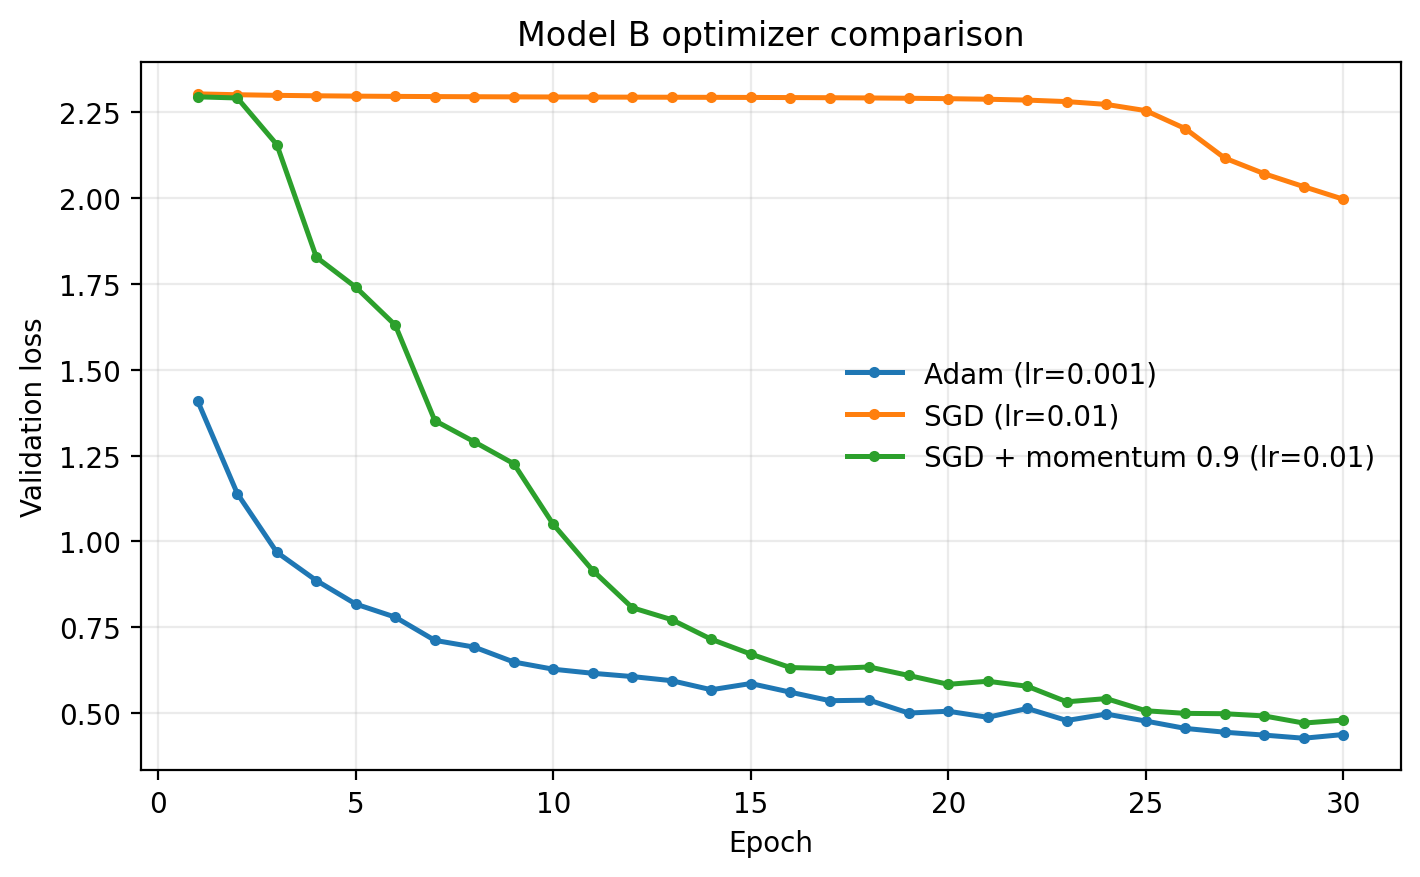
\includegraphics[width=0.86\linewidth]{figures/optimizer_comparison.png}
  \caption{Validation-loss comparison for Adam, plain SGD, and SGD with
  momentum on Model~B under an otherwise identical training budget.}
  \label{fig:optimizer-comparison}
\end{figure}

\subsection{Effect of the momentum coefficient}
\label{sec:momentum-ablation}

We compared SGD with $m\in\{0,0.5,0.9,0.99\}$ at the fixed learning
rate $\alpha=10^{-2}$.  The split, seed, data order, augmentation, batch size,
initialisation and 30-epoch budget were identical.  All four runs used an
NVIDIA GeForce RTX~3060 Laptop GPU.  Figure~\ref{fig:momentum-ablation}
uses the separate \texttt{momentum\_m000}, \texttt{momentum\_m050},
\texttt{momentum\_m090}, and \texttt{momentum\_m099} records.  Their epoch
times cannot be compared directly with the T4 runs in
Table~\ref{tab:optimizer-comparison}.

In the momentum update,
\begin{equation}
  v \leftarrow mv-\alpha\frac{\partial L(w)}{\partial w},
  \qquad w \leftarrow w+v,
  \label{eq:momentum-update}
\end{equation}
$m$ determines how much of the previous velocity is kept.  Gradients with a
consistent sign accumulate in $v$, increasing movement in that direction.
Across a narrow loss ravine, alternating gradient components cancel part of
the stored velocity, damping side-to-side motion.

With $m=0$, the update has no memory and validation loss stays high over the
epoch budget.  At $m=0.5$, loss falls sooner but is still high after 30 epochs.
At $m=0.9$, validation loss falls with small epoch-to-epoch fluctuations
and reaches the lowest value.  At $m=0.99$, loss falls fastest initially,
then fluctuates during later epochs and finishes above its selected minimum.
Keeping more past velocity could explain these fluctuations, but the saved
loss curves do not record gradient directions or establish overshooting.

We selected $m=0.9$ by validation loss.  The slightly higher test accuracy
at $m=0.99$ did not affect that choice.  This ranking is based on one run per
setting; its consistency across random seeds has not been measured.

\begin{figure}[H]
  \centering
  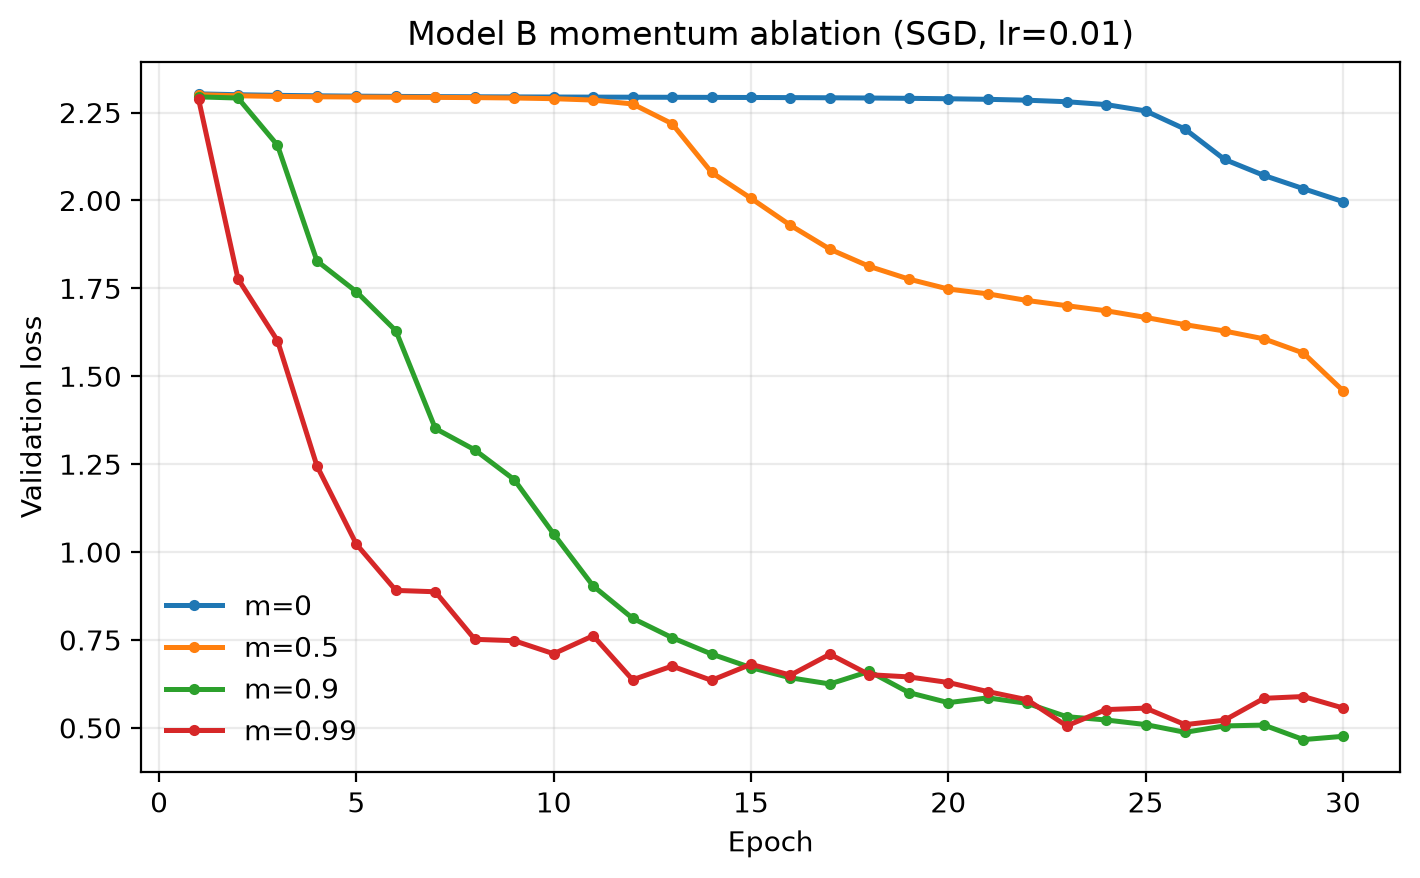
\includegraphics[width=0.86\linewidth]{figures/momentum_ablation.png}
  \caption{Validation-loss curves for Model~B with SGD at
  $\alpha=10^{-2}$.  Momentum is the only methodological variable across the
  four 30-epoch runs.}
  \label{fig:momentum-ablation}
\end{figure}
          % #13, #14: optimizer comparison, momentum

% =========================================================================
\section{Task 4: Custom Model Training and Evaluation}
\label{sec:task4}

\subsection{Custom-model training and evaluation}
\label{sec:custom-results}

Both custom networks were trained for 30 epochs with Adam on the same
stratified split, random seed, augmentation pipeline, batch size, and Tesla
T4 device.  Checkpoint selection used the lowest validation loss, and the test
split was evaluated only after that selection.  Figure~\ref{fig:custom-loss}
therefore compares like with like rather than mixing devices or training
budgets.

\begin{figure}[htbp]
  \centering
  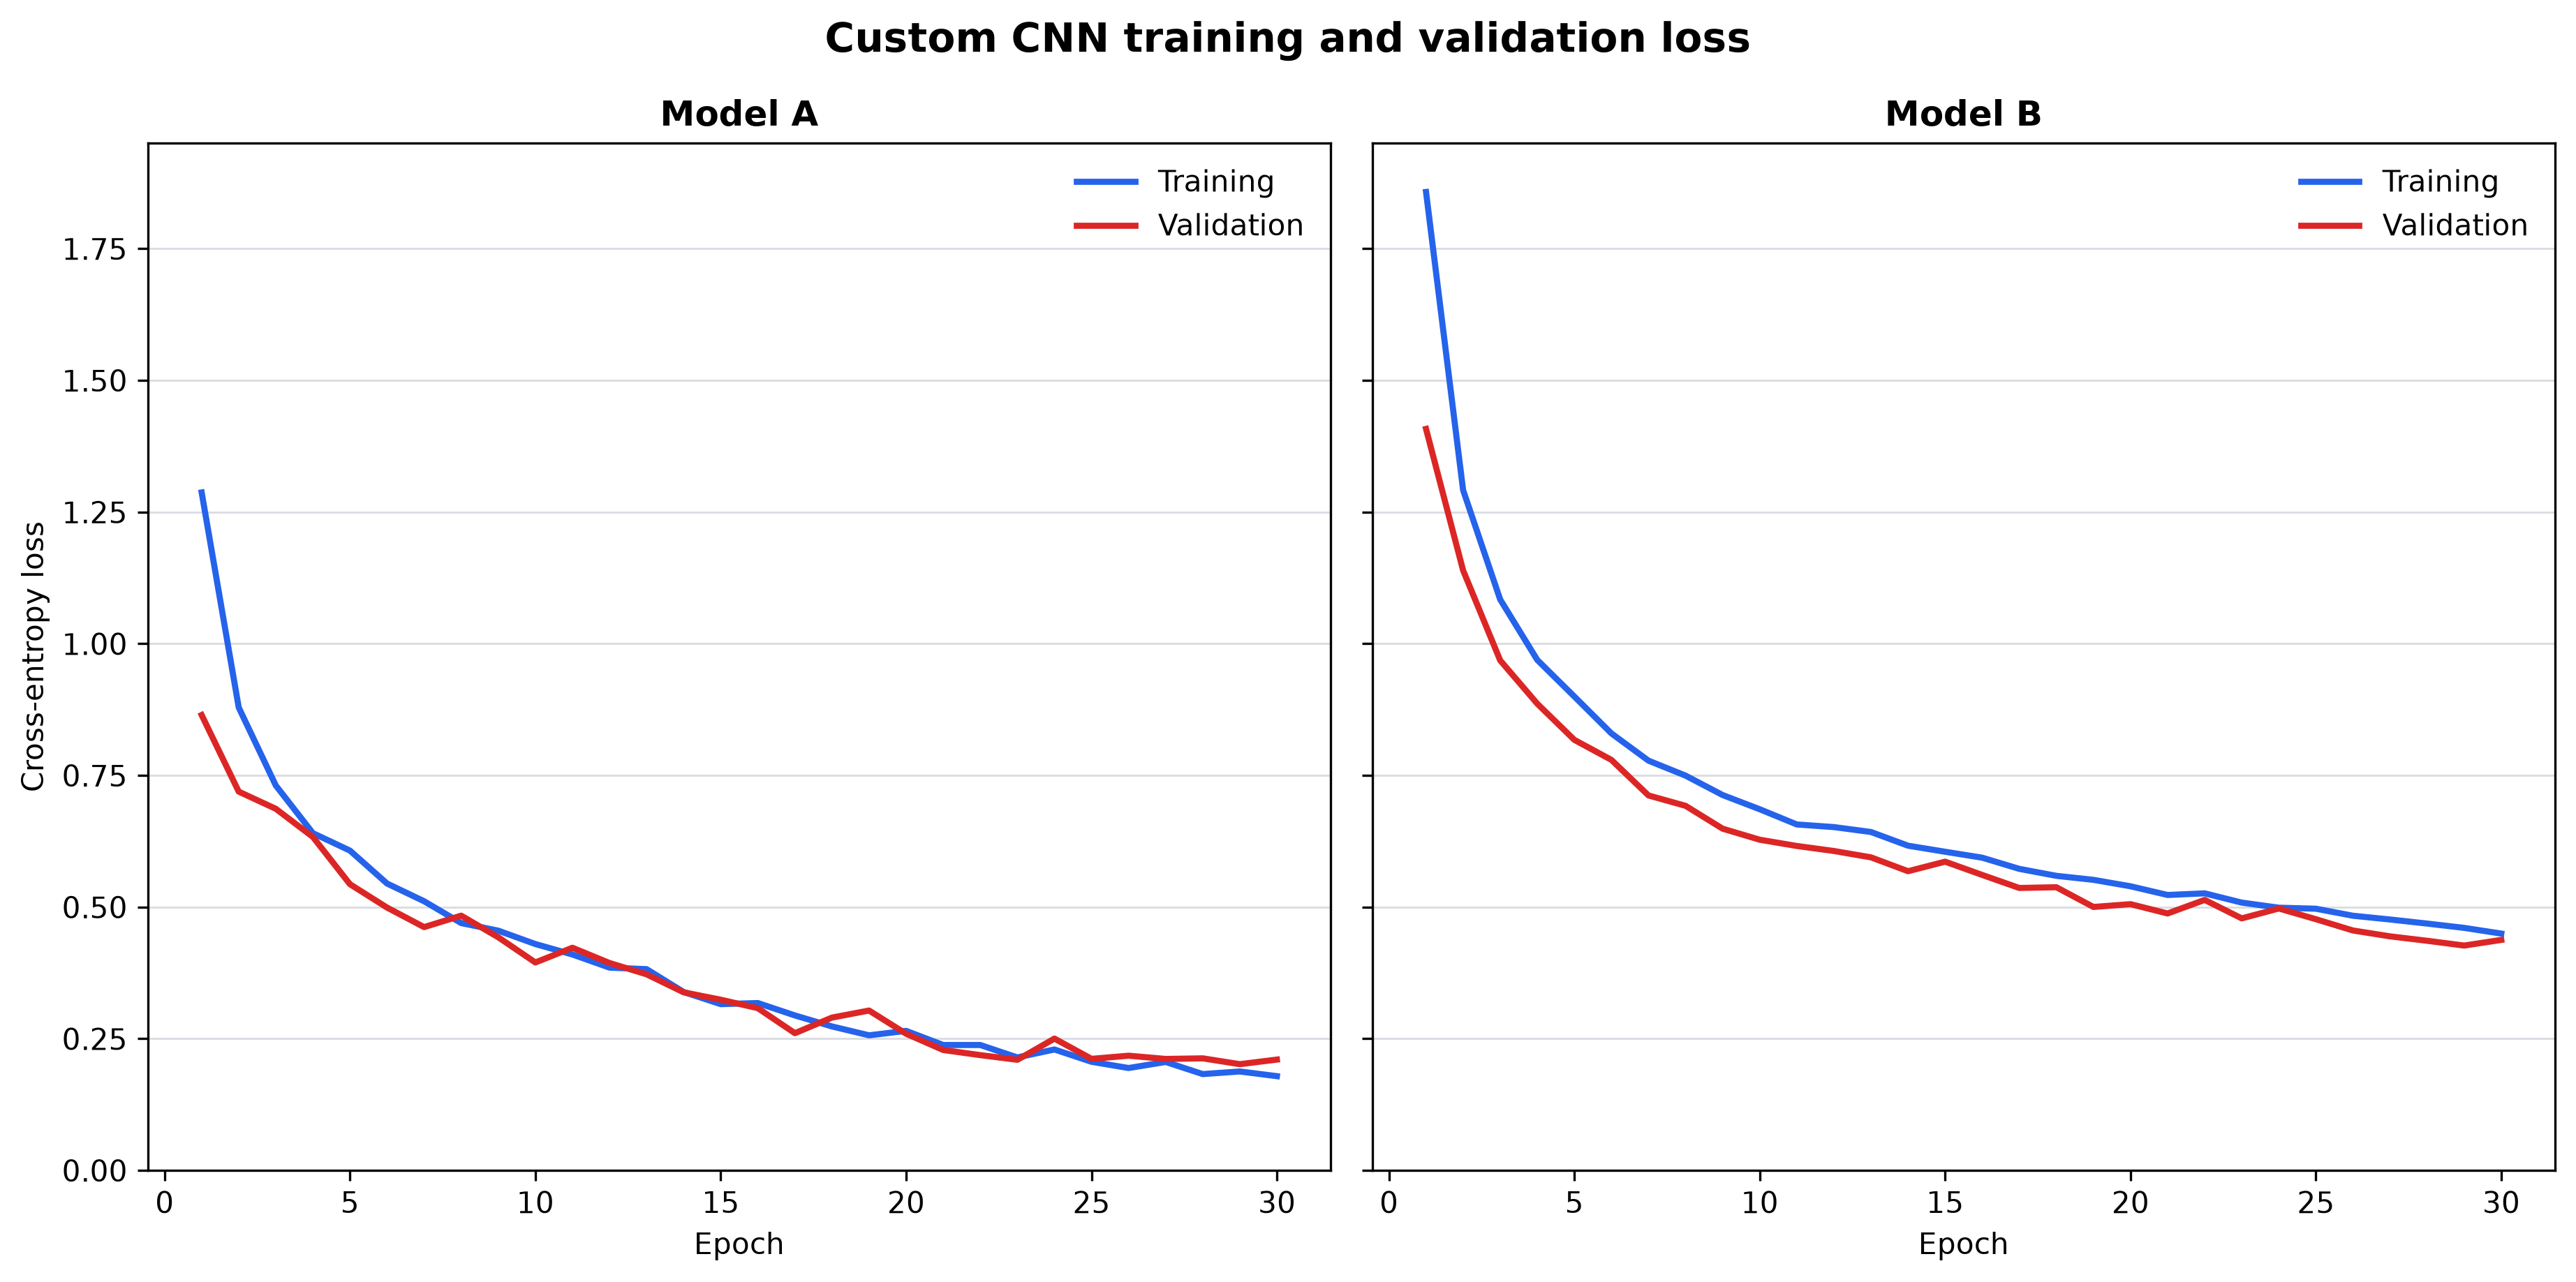
\includegraphics[width=\linewidth]{figures/custom_loss_curves.png}
  \caption{Training and validation cross-entropy loss for Model~A and
  Model~B.  The panels share a common vertical scale.}
  \label{fig:custom-loss}
\end{figure}

\begin{table}[htbp]
  \centering
  \small
  \resizebox{\linewidth}{!}{\begin{tabular}{lrrrrrr}
\hline
Model & Parameters & Size (KB) & Epoch (s) & Accuracy (\%) & Precision (\%) & Recall (\%) \\
\hline
Model A & 692{,}106 & 2{,}708.06 & 11.80 & 92.89 & 93.20 & 92.52 \\
Model B & 36{,}968 & 150.98 & 11.61 & 83.75 & 83.30 & 83.42 \\
\hline
\end{tabular}
}
  \caption{Custom-model comparison generated from the committed test metrics
  and profiler outputs.  Precision and recall are macro averages over the ten
  EuroSAT classes; epoch time was measured on the same Tesla T4.}
  \label{tab:custom-comparison}
\end{table}

Table~\ref{tab:custom-comparison} shows the central resource--accuracy
trade-off.  Replacing standard convolutions with depthwise and pointwise steps,
and replacing the flattened classifier input with global average pooling,
makes Model~B dramatically smaller while giving up some test accuracy, macro
precision, and macro recall.  The reduced capacity is most visible for
visually overlapping land-cover categories: Figure~\ref{fig:model-b-confusion}
shows more confusion among Herbaceous Vegetation, Permanent Crop, Highway,
and River than Figure~\ref{fig:model-a-confusion}.  In contrast, both models
remain strong on classes with more distinctive appearance, including Forest,
Residential, and Sea/Lake.

\subsubsection{Convergence control}

The 30-epoch comparison controls the early training budget, but its loss curve
shows that Model~B had not converged.  To separate convergence speed from
architecture capability, both models were therefore repeated for 100 epochs
with otherwise identical configurations.  The first 30 loss and accuracy
records reproduce the original runs exactly (apart from wall-clock noise), so
this is a controlled extension rather than a new hyperparameter search.

\begin{figure}[htbp]
  \centering
  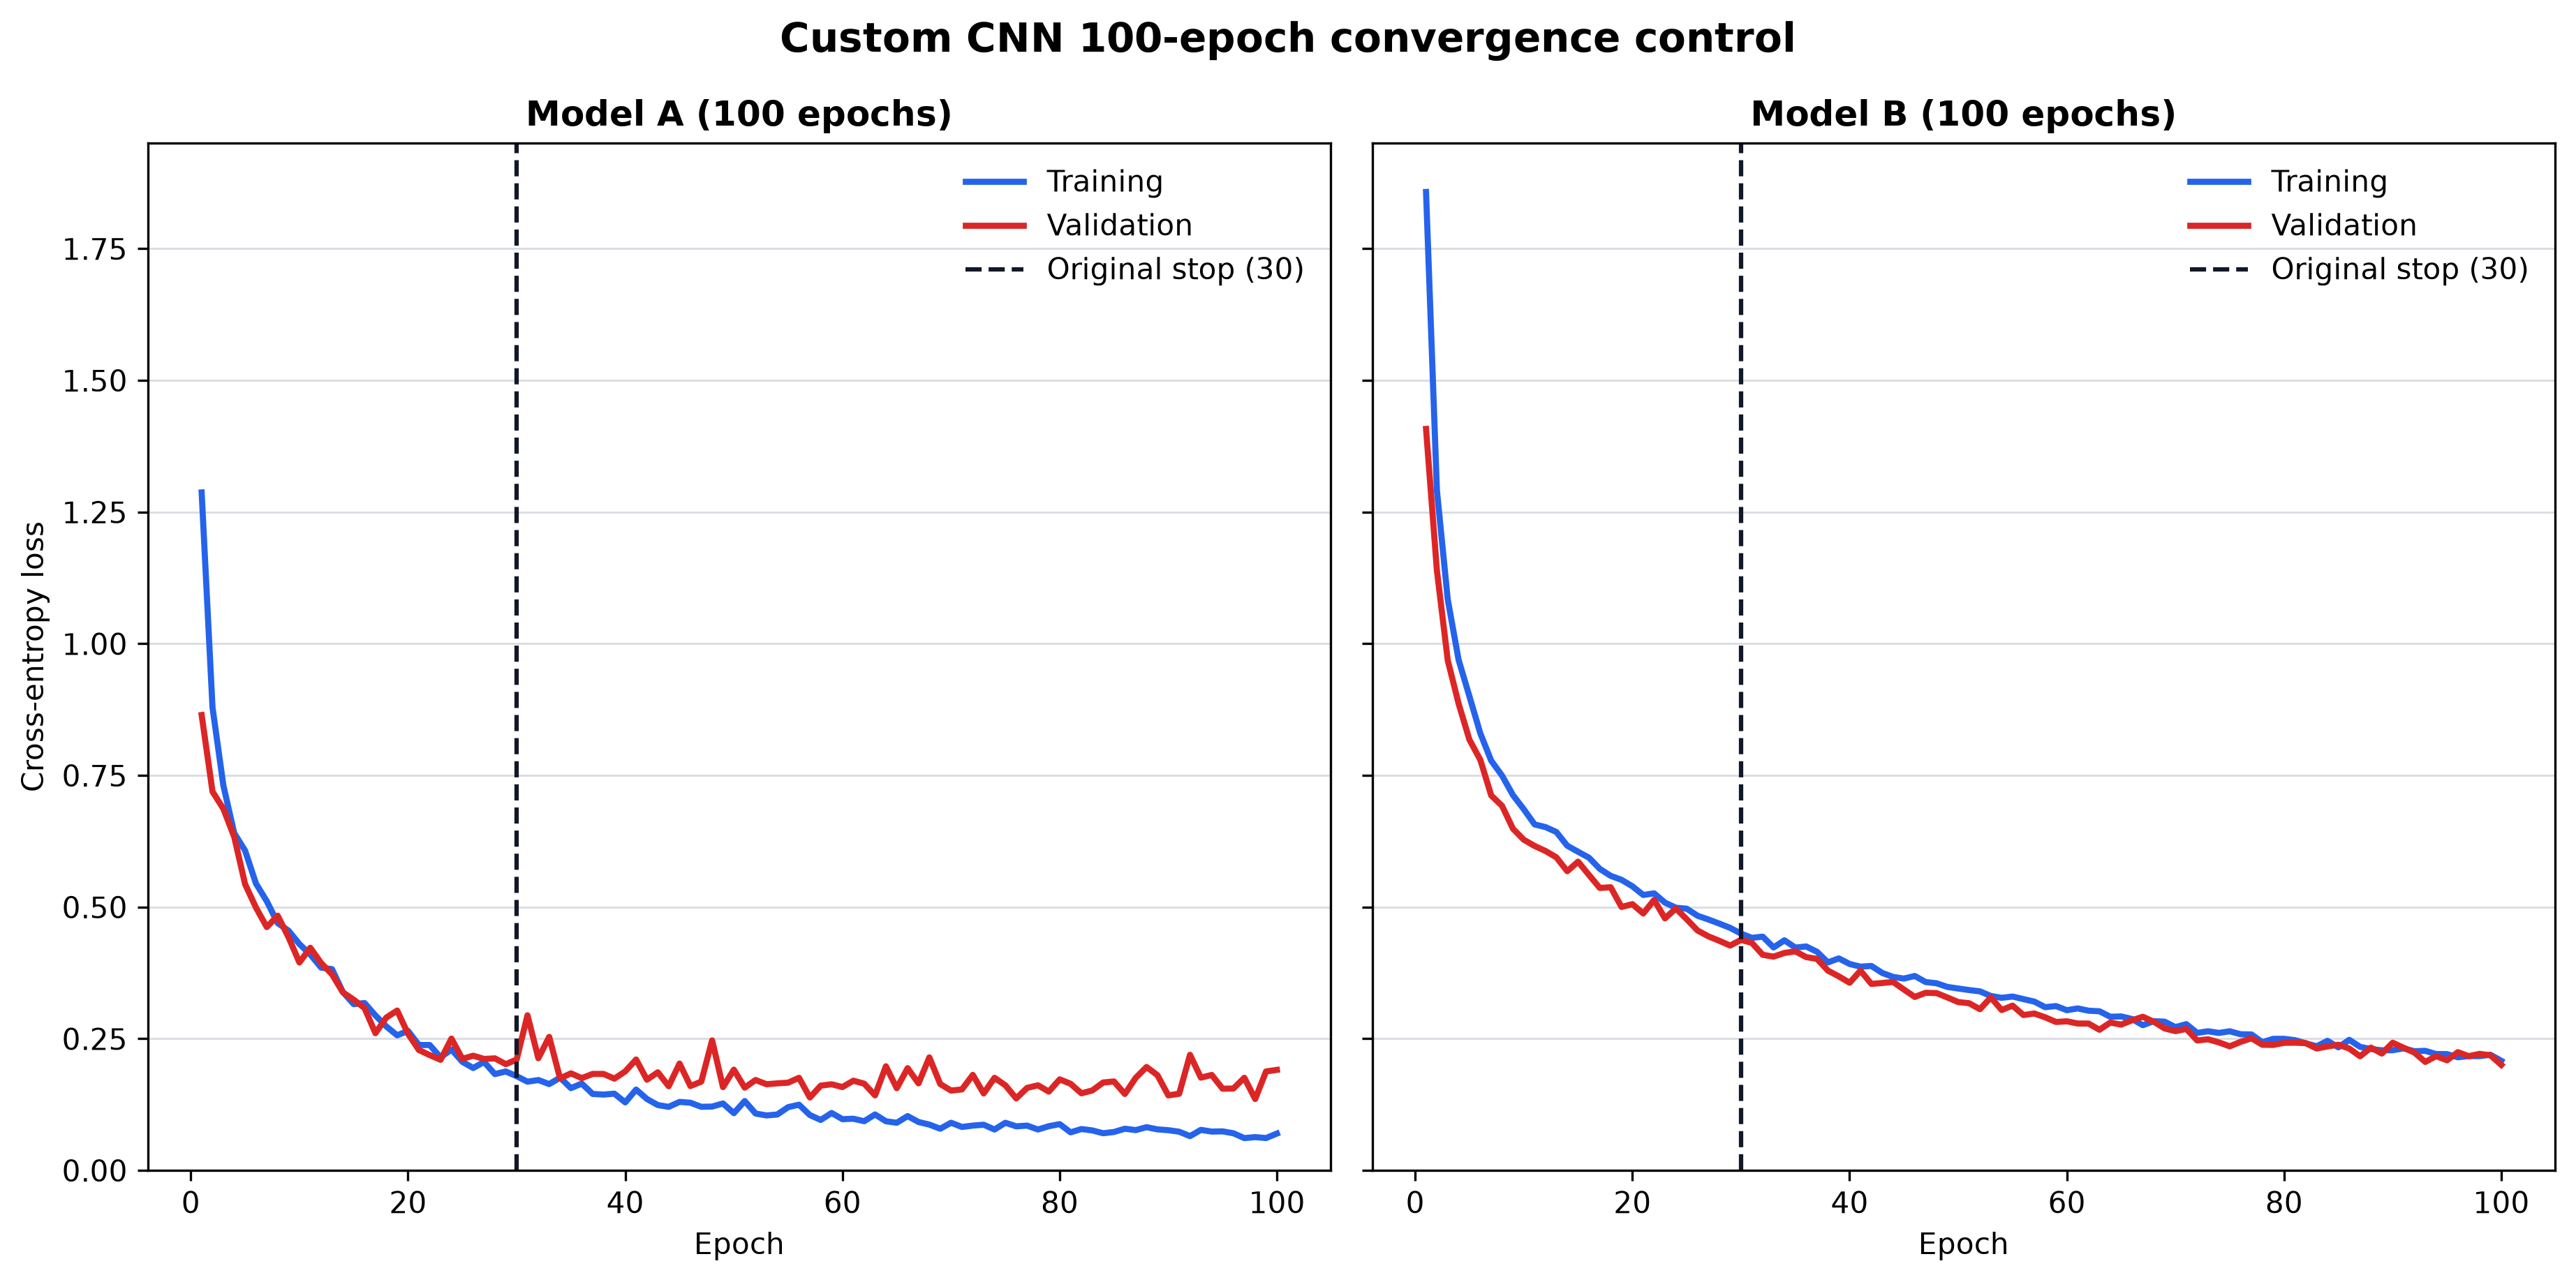
\includegraphics[width=\linewidth]{figures/custom_convergence.png}
  \caption{One-hundred-epoch training and validation loss for both custom
  models.  The dashed line marks the original 30-epoch stopping point.}
  \label{fig:custom-convergence}
\end{figure}

\begin{table}[htbp]
  \centering
  \scriptsize
  \resizebox{\linewidth}{!}{\begin{tabular}{lrrrrrrrrr}
\hline
Model & Epochs & Selected & Best val. loss & Best val. acc. (\%) & Test acc. (\%) & Parameters & Size (KB) & MACs & Epoch (s) \\
\hline
Model A & 30 & 29 & 0.2018 & 93.43 & 92.89 & 692{,}106 & 2{,}708.06 & 30{,}038{,}016 & 11.80 \\
Model A & 100 & 98 & 0.1355 & 96.00 & 96.00 & 692{,}106 & 2{,}708.06 & 30{,}038{,}016 & 12.54 \\
Model B & 30 & 29 & 0.4270 & 84.42 & 83.75 & 36{,}968 & 150.98 & 3{,}725{,}196 & 11.61 \\
Model B & 100 & 100 & 0.2004 & 93.26 & 93.14 & 36{,}968 & 150.98 & 3{,}725{,}196 & 12.29 \\
\hline
\end{tabular}
}
  \caption{Controlled custom-model convergence comparison.  ``Selected'' is
  the lowest-validation-loss checkpoint; all timings were measured on the
  same Tesla T4.}
  \label{tab:custom-convergence}
\end{table}

Table~\ref{tab:custom-convergence} shows that longer training benefits
Model~B much more strongly, substantially narrowing the accuracy gap without
changing its parameter, storage, or MAC advantage.  The two tables answer
different questions: Table~\ref{tab:custom-comparison} measures performance
under the same early epoch budget, whereas Table~\ref{tab:custom-convergence}
measures the architectures after a longer equal budget.  The former must not
be presented as Model~B's converged capability.

Model~A shows mild late-stage overfitting: its training loss continues to
fall while validation loss plateaus and fluctuates.  Selecting the
lowest-validation-loss checkpoint at epoch 98 mitigates that deterioration,
and the matching validation and test accuracies support good generalisation
of the selected checkpoint.  Model~B selects the final epoch, so even the
100-epoch result should be described as the achieved result, not a proven
upper limit on the architecture.

\begin{figure}[htbp]
  \centering
  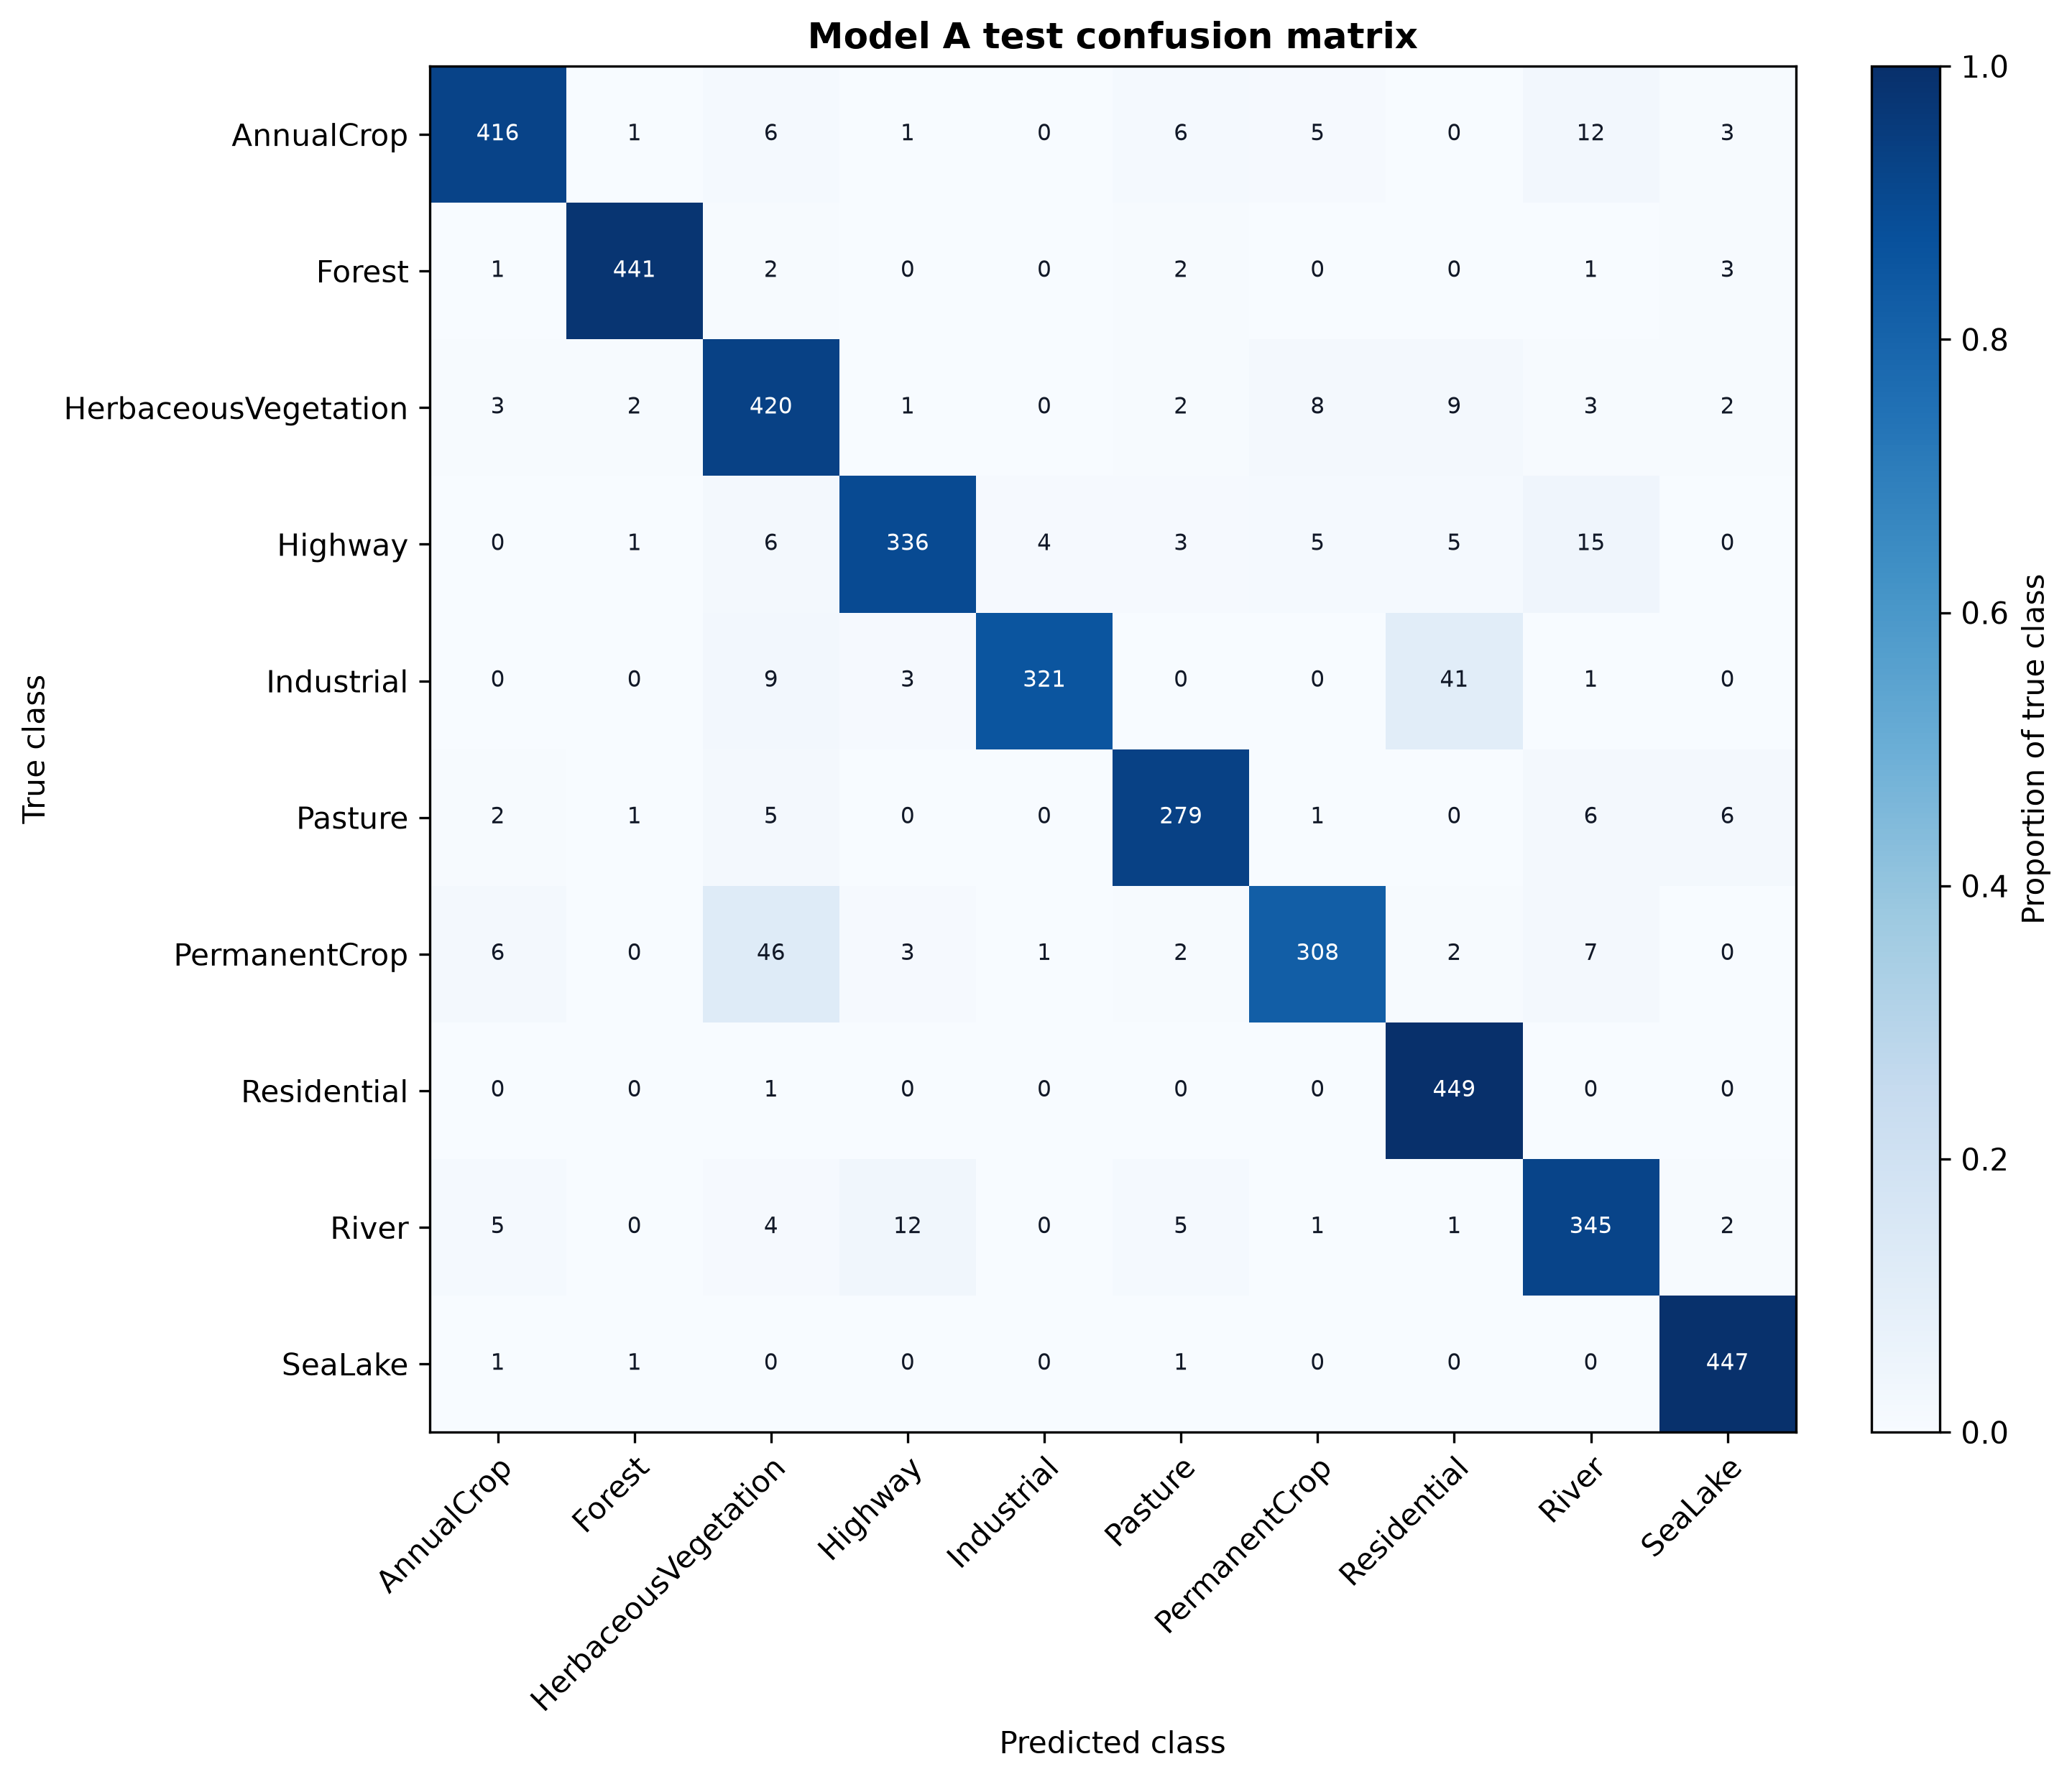
\includegraphics[width=0.82\linewidth]{figures/model_a_confusion_matrix.png}
  \caption{Model~A test confusion matrix.  Colour is normalised within each
  true-class row and annotations give raw sample counts.}
  \label{fig:model-a-confusion}
\end{figure}

\begin{figure}[htbp]
  \centering
  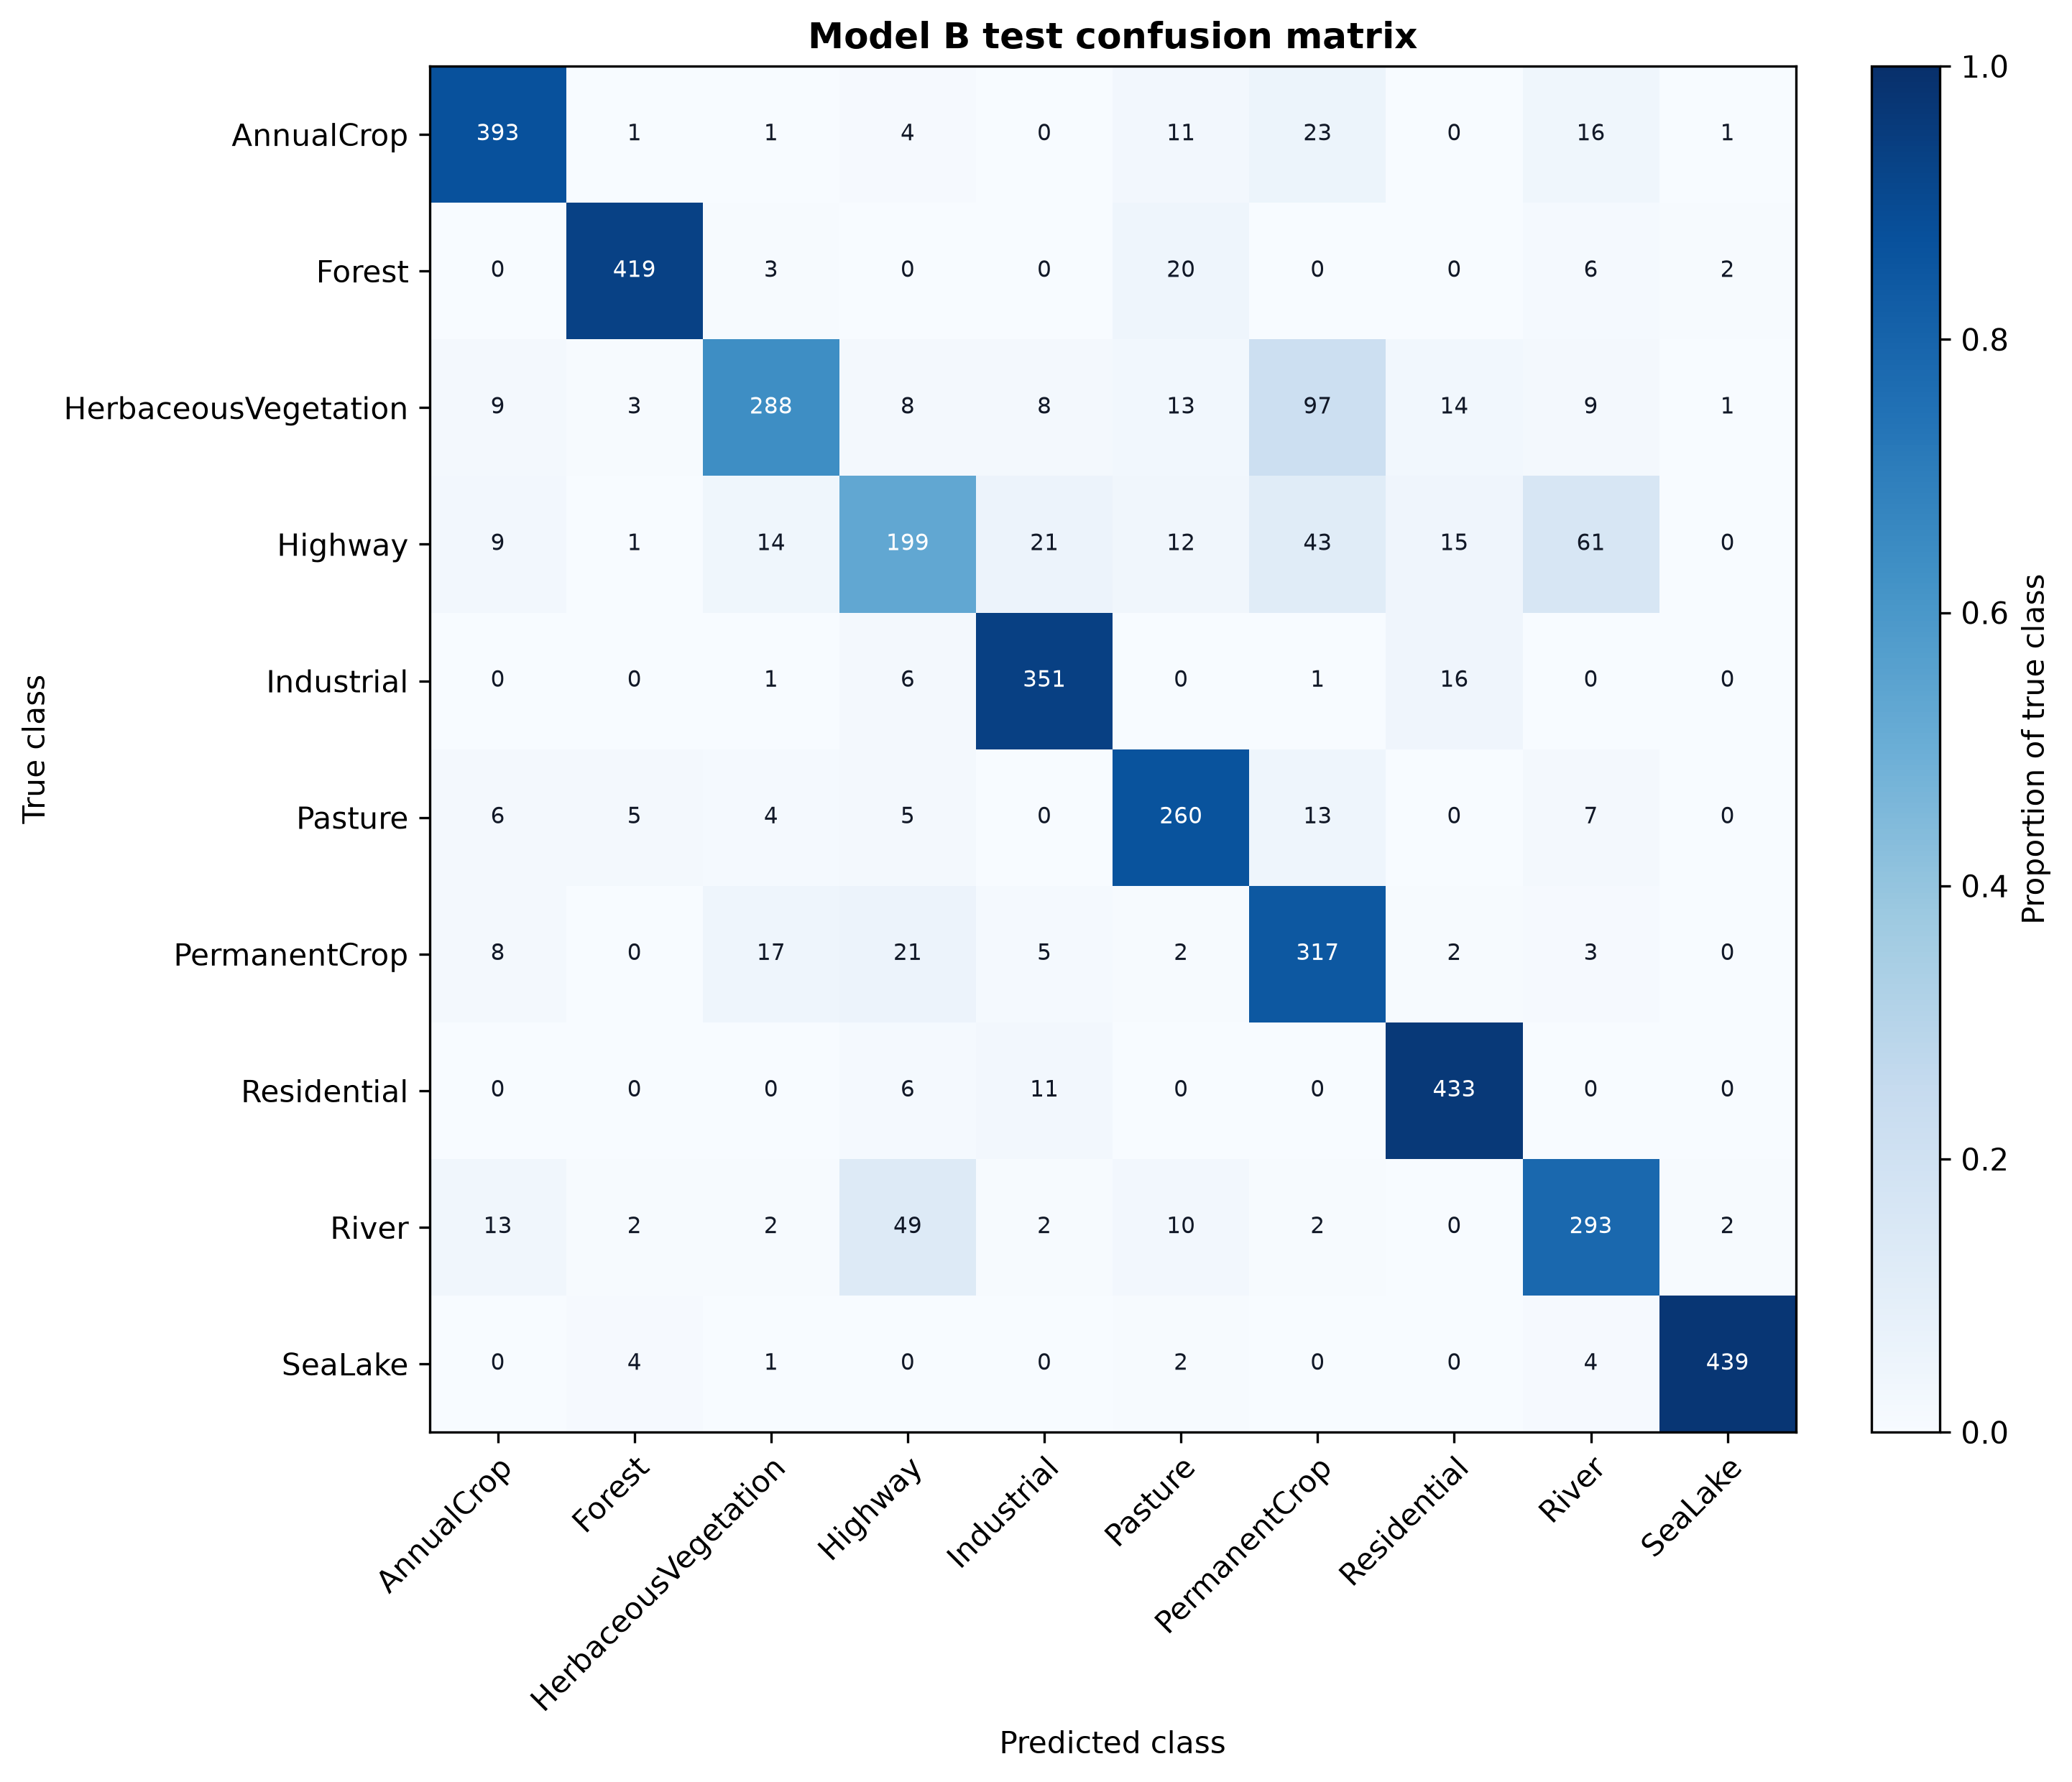
\includegraphics[width=0.82\linewidth]{figures/model_b_confusion_matrix.png}
  \caption{Model~B test confusion matrix, using the same convention as
  Figure~\ref{fig:model-a-confusion}.}
  \label{fig:model-b-confusion}
\end{figure}

The storage saving is substantial, but the epoch-time reduction is small.
This is not a contradiction: the profiler counts arithmetic, whereas wall-clock
training also includes data loading, augmentation, framework overhead, memory
traffic, and the efficiency of the accelerator's particular convolution
kernels.  Depthwise convolution reduces theoretical work without guaranteeing
the same proportional speed-up on a highly parallel GPU.  Its benefit is
clearer under the assignment's edge constraint, where the much smaller
parameter footprint and lower MAC count directly reduce storage and inference
work.  Model~A is preferable when predictive performance is the priority;
Model~B is the defensible choice when the parameter ceiling and deployability
are hard constraints.
     % #15-#18: training, evaluation, A vs B

% =========================================================================
\section{Task 5: Lightweight State-of-the-Art Models}
\label{sec:task5}

% Owned by #22 (SOTA metrics table), with results from #20 (MobileNetV2) and
% #21 (EfficientNet-B0). Every number is in tables/sota_comparison.tex,
% generated by scripts/build_tables.py --table sota - none is typed here.

\subsection{Transfer-learning protocol}
\label{sec:sota-protocol}

Two pretrained architectures were adapted to EuroSAT:
MobileNetV2~\cite{sandler2018mobilenetv2}, and EfficientNet-B0~\cite{tan2019efficientnet}.
Both start from ImageNet weights and the final linear layer of each classifier was replaced by a
new ten-class prediction layer. Every run uses the same stratified split as the Models A and B, 
random seed, augmentation, training-split normalisation statistics, batch
size of 128, 30-epoch budget and Colab Tesla~T4 as the machine to run on. 
The checkpoint was chosen by lowest validation loss, before testing.

Once the new prediction layer is in place, there were two cases to choose from, either
keep the pretrained backbone \emph{frozen}, or \emph{fine-tune} it. Each
network was tested using both methods, to decide wether there is a gain by fine tuning all parameters.

\begin{itemize}[leftmargin=*]
  \item \textbf{Frozen.} In this case, only the new prediction layer was trained, with Adam Optimizer at
  a learning rate of $10^{-3}$. The CNN backbone acts as a fixed feature extractor,
  and its batch-normalisation statistics were held at their original ImageNet values.
  \item \textbf{Fine-tuned.} In this case, every weight was trained, starting from the
  ImageNet weights, with Adam at a learning rate of $10^{-4}$. Here we chose a learning rate
  below the frozen-backbone rate to limit changes to the pretrained filters while
  the new classifier learns.
\end{itemize}

Our main runs keep the input at $64\times64$,which is the original resolution that the custom
models see. Because ImageNet networks are
designed for $224\times224$ input, the experiment was repeated for each network
with the $64\times64$ images upsampled to $224\times224$, for both the frozen and fine-tuned cases. Each $224\times224$
pair differs from its original pair in input size only, so as to identify the effect of the original resolution on the pretrained features.

\subsection{Results}
\label{sec:sota-results}

\begin{table}[htbp]
  \centering
  % Nine columns: set small rather than \resizebox-ed, because the Pending
  % box \generatedtable shows before the runs exist cannot sit in a \resizebox.
  \footnotesize
  \setlength{\tabcolsep}{4pt}
  \generatedtable{tables/sota_comparison.tex}{\#22}
  \caption{Pretrained lightweight models on the EuroSAT test split. Precision
  and recall are averages over the ten classes. \emph{Trained} counts the
  parameters updated during training. Sizes are in MB, measured from the saved
  weights; the custom models in Table~\ref{tab:custom-comparison} are in KB.
  The rows under Supplementary section upsample the $64\times64$ images to $224\times224$.}
  \label{tab:sota-comparison}
\end{table}

Table~\ref{tab:sota-comparison} lists the results from both cases for each network. \emph{Parameters} and \emph{Size} are
identical for the frozen and fine-tuned runs of a network, because freezing
changes what is trained, not what is deployed. \emph{Trained} is where they
differ.  In the frozen case it updates only the prediction layer,which is under one
per cent of the network. Accuracy
gaps between the two rows of a pair is therefore bought with training effort
alone, with no cost in memory.

We observed that for both networks that accuracy gap is large. Fine-tuning raises all the metrics by 5--10 points
above the frozen feature extractor CNN case. The explanation is likely the domain shift from ImageNet to Satellite Images.
ImageNet filters were learnt on close-range photographs of objects, while
EuroSAT is overhead satellite images at a much larger scale. 
A frozen backbone can only re-weight features that were learnt for the wrong kind of
image while fine-tuning lets the filters themselves move towards field boundaries,
road textures and water.

The two architectures also rank differently under the two strategies described above. Frozen,
EfficientNet-B0 is clearly the weaker network, despite having almost twice
MobileNetV2's parameters. In the Fine-tuned case, the two networks are practically at the same level. The
gap between them therefore says how well each network's ImageNet features happen to
transfer to $64\times64$ overhead images.
At $64\times64$, both networks' downsampling stages leave a $2\times2$ final
feature map. Different sensitivity of the pretrained features to input
scale is a possible explanation.
Once fine-tuned, however, EfficientNet-B0 offers no meaningful accuracy over
MobileNetV2 for nearly twice the memory. Therefore MobileNetV2 is the better edge
candidate of the two.

The supplementary rows show that upsampling to $224\times224$ gives both frozen backbones a gain of
several points, but the fine-tuned models gain less than one. A possible explanation for this is the fact that frozen
network's filters are fixed at ImageNet's scale, so enlarging the input
is the only way to bring the data to them. Fine-tuning instead moves the
filters to the data, after which resolution matters much less: for each
network, the fine-tuned $64\times64$ model outperforms the frozen
$224\times224$ one. It also does about $(224/64)^2\approx12$ times fewer
operations per image, because a convolution's cost scales with the $H\times W$
of its output. For an edge device,
fine-tuning at native resolution is the cheaper way to get accuracy.

Even the smallest of these models is one to two orders of magnitude larger on
disk than Model~B (Table~\ref{tab:custom-comparison}). Whether the extra accuracy is worth that memory is the
question Section~\ref{sec:task6} answers.

The training curves (Figures~\ref{fig:sota-loss}--\ref{fig:efficientnet-224-loss})
show the split between the two strategies for both networks. Each frozen
run levels off at a clearly higher loss than its fine-tuned partner. At
$64\times64$ the frozen runs' training and validation losses stay close
together. The frozen
EfficientNet-B0 curves are also visibly noisier than MobileNetV2's: after the
first few epochs both of its losses fluctuate instead of
settling, and at $224\times224$ the lowest validation loss happens to fall early,
so its selected checkpoint comes early in the run. The fine-tuned curves of
both networks are smooth and settle within a few epochs.

The noise in the frozen EfficientNet-B0 curves comes from its fixed features,
not from a training fault. While its validation loss swings from epoch to
epoch, its validation accuracy stays almost level, so the predicted classes
barely change; what changes is the confidence given to the many images that
the frozen features do not separate. Cross-entropy penalises a confidently
wrong prediction heavily, so small updates to the prediction layer move the
loss on these borderline images far more than they move the accuracy.
MobileNetV2's frozen features leave fewer such images, and its loss is lower
and flatter. The two backbones also end in different activations.
EfficientNet-B0 uses the unbounded SiLU (Swish)
activation~\cite{tan2019efficientnet}, and a small fraction of images produce
very large pooled features. 
MobileNetV2's ReLU6 caps every feature at
six~\cite{sandler2018mobilenetv2}, the bounded behaviour discussed in
Section~\ref{sec:activation-choice}. In a diagnostic check that retrained only the prediction
layer on fixed features, standardising those features reduced the
fluctuation only slightly. Learning rates of $3\times10^{-4}$ and $10^{-4}$
did not remove it either, so the frozen-head learning rate is not the cause.
The practical cost lies in checkpoint selection. On a noisy validation curve
the lowest-loss epoch is partly a matter of chance, and it need not be the
run's most accurate epoch. Fine-tuning removes the effect because the backbone
adapts its features to EuroSAT, which is one more reason the comparison in
Section~\ref{sec:task6} uses the fine-tuned runs.

The confusion matrices of the fine-tuned models
(Figures~\ref{fig:mobilenetv2-confusion}--\ref{fig:efficientnet-224-confusion})
place the remaining errors in the same few class pairs for both networks.
Highway and River are confused in both directions; at $64\times64$ both are
thin linear features a few pixels wide. The agricultural and vegetation
classes (AnnualCrop, PermanentCrop, Pasture and HerbaceousVegetation), which
differ mainly in texture, account for a large share of the rest.

\begin{figure}[htbp]
  \centering
  \generatedfigure{figures/sota_loss_curves.png}{\#20}
  \caption{Training and validation loss of MobileNetV2 at $64\times64$, with
  the backbone frozen and fine-tuned.}
  \label{fig:sota-loss}
\end{figure}

\begin{figure}[htbp]
  \centering
  \generatedfigure{figures/efficientnet_loss_curves.png}{\#64}
  \caption{Training and validation loss of EfficientNet-B0 at $64\times64$,
  with the backbone frozen and fine-tuned.}
  \label{fig:efficientnet-loss}
\end{figure}

\begin{figure}[htbp]
  \centering
  \generatedfigure{figures/sota_224_loss_curves.png}{\#20}
  \caption{Training and validation loss of MobileNetV2 at $224\times224$ (the
  supplementary resolution ablation), with the backbone frozen and fine-tuned.}
  \label{fig:sota-224-loss}
\end{figure}

\begin{figure}[htbp]
  \centering
  \generatedfigure{figures/efficientnet_224_loss_curves.png}{\#64}
  \caption{Training and validation loss of EfficientNet-B0 at $224\times224$
  (the supplementary resolution ablation), with the backbone frozen and
  fine-tuned.}
  \label{fig:efficientnet-224-loss}
\end{figure}

\begin{figure}[htbp]
  \centering
  \generatedfigure[width=0.82\linewidth]{figures/mobilenetv2_64_ft_confusion_matrix.png}{\#20}
  \caption{Test confusion matrix of the fine-tuned MobileNetV2 at $64\times64$.}
  \label{fig:mobilenetv2-confusion}
\end{figure}

\begin{figure}[htbp]
  \centering
  \generatedfigure[width=0.82\linewidth]{figures/efficientnetb0_64_ft_confusion_matrix.png}{\#64}
  \caption{Test confusion matrix of the fine-tuned EfficientNet-B0 at
  $64\times64$.}
  \label{fig:efficientnet-confusion}
\end{figure}

\begin{figure}[htbp]
  \centering
  \generatedfigure[width=0.82\linewidth]{figures/efficientnetb0_224_ft_b128_confusion_matrix.png}{\#64}
  \caption{Test confusion matrix of the fine-tuned EfficientNet-B0 at
  $224\times224$ (supplementary).}
  \label{fig:efficientnet-224-confusion}
\end{figure}
       % #20-#22: fine-tuned SOTA results

% =========================================================================
% Finish Task 5's figures before starting the final discussion.
\clearpage
\section{Task 6: Final Comparison and Trade-offs}
\label{sec:task6}

% Owned by #25 (task 6 final comparison and trade-off discussion), the
% largest single writing deliverable (20 marks). Stub created by #23.
%
% To write: Model B against the fine-tuned SOTA models on accuracy, memory
% footprint and computational cost, and the trade-offs of a custom sub-100k
% model trained from scratch versus an industry-standard pretrained one. The
% edge argument is analytic: MACs, size in KB, and what fits in a
% microcontroller's SRAM.

\subsection{Model B against lightweight SOTA models}
\label{sec:final-comparison}

\begin{table}[htbp]
  \centering
  \caption{Model B against the fine-tuned SOTA models: accuracy, parameters,
  size, MACs and training time per epoch.}
  \label{tab:final-comparison}
  \generatedtable{tables/final_comparison.tex}{\#25}
\end{table}

\subsection{Trade-offs: accuracy, memory and compute}
\label{sec:trade-offs}

\pending{trade-off discussion: accuracy vs memory footprint vs computational
cost, and custom-from-scratch vs pretrained (\#25)}

\subsection{Conclusion}
\label{sec:conclusion}

\pending{conclusion (\#25)}
         % #25: Model B vs SOTA

% =========================================================================
\appendix
\section{Generated Layer Tables}
\label{app:layer-tables}

The per-layer tables below are produced by
\texttt{scripts/build\_tables.py} directly from the model definitions, by a
forward pass of one $64\times64$ image. They are the machine-generated
counterpart of the hand derivations in Section~\ref{sec:task2}: every
parameter count there must match the corresponding row here.

\begin{table}[H]
  \centering
  \caption{Model A layer summary, generated from \texttt{configs/model\_a.yaml}.}
  \label{tab:model-a-layers}
  \generatedtable{tables/model_a_layers.tex}{\#9}
\end{table}

\begin{table}[H]
  \centering
  \caption{Model B layer summary, generated from \texttt{configs/model\_b.yaml}.
  Each depthwise separable block appears as its two steps.}
  \label{tab:model-b-layers}
  \generatedtable{tables/model_b_layers.tex}{\#10}
\end{table}

% =========================================================================
% References (#72): IEEE style, numbered in order of first citation. After
% the appendix, as in IEEE papers; listed in the table of contents.
\clearpage
\phantomsection
\addcontentsline{toc}{section}{References}
% References in IEEE style (#72), input at the end of main.tex.
%
% IEEE numbers references in order of FIRST CITATION in the document, and
% thebibliography numbers them in the order listed here - so the \bibitem
% order below must follow the order of first \cite in the report. A new
% citation goes in at the position of its first use, not at the end.
% tests/test_report.py enforces the order, and that every \cite has an entry
% and every entry is cited.
%
% thebibliography rather than BibTeX: two plain pdflatex passes resolve every
% citation, so the report builds the same way in CI (latexmk), in VS Code and
% with pdflatex run directly, with no bibtex step to forget.
%
% Bibliographic details verified on 19 Oct 2026 against Crossref (DOIs),
% arXiv and PMLR; web sources were opened on that date where they allow it.

\begin{thebibliography}{99}

\bibitem{helber2019eurosat}
P.~Helber, B.~Bischke, A.~Dengel, and D.~Borth, ``EuroSAT: A novel dataset
and deep learning benchmark for land use and land cover classification,''
\emph{IEEE J. Sel. Topics Appl. Earth Observ. Remote Sens.}, vol.~12, no.~7,
pp.~2217--2226, Jul. 2019, doi: 10.1109/JSTARS.2019.2918242.

\bibitem{torchvision2016}
TorchVision maintainers and contributors, ``TorchVision: PyTorch's computer
vision library,'' GitHub repository, 2016. [Online]. Available:
\url{https://github.com/pytorch/vision}. Accessed: Oct.~19, 2026.

\bibitem{deng2009imagenet}
J.~Deng, W.~Dong, R.~Socher, L.-J.~Li, K.~Li, and L.~Fei-Fei, ``ImageNet: A
large-scale hierarchical image database,'' in \emph{Proc. IEEE Conf. Comput.
Vis. Pattern Recognit. (CVPR)}, Miami, FL, USA, 2009, pp.~248--255,
doi: 10.1109/CVPR.2009.5206848.

\bibitem{cmsisnn}
Arm Ltd., ``CMSIS-NN software library,'' GitHub repository.
Revision \texttt{71cbe3d5a686c875c88a4d112633b13fae94b5a2}. [Online].
Available: \url{https://github.com/ARM-software/CMSIS-NN/tree/71cbe3d5a686c875c88a4d112633b13fae94b5a2}.
Accessed:
Oct.~19, 2026.

\bibitem{arm2016dsp}
Arm Ltd., ``White paper: DSP capabilities of Cortex-M4 and Cortex-M7,'' Arm
Community Blogs, 2016. [Online]. Available:
\url{https://developer.arm.com/community/arm-community-blogs/b/architectures-and-processors-blog/posts/white-paper-dsp-capabilities-of-cortex-m4-and-cortex-m7}

\bibitem{hendrycks2016gelu}
D.~Hendrycks and K.~Gimpel, ``Gaussian error linear units (GELUs),'' 2016,
arXiv:1606.08415.

\bibitem{sandler2018mobilenetv2}
M.~Sandler, A.~Howard, M.~Zhu, A.~Zhmoginov, and L.-C.~Chen, ``MobileNetV2:
Inverted residuals and linear bottlenecks,'' in \emph{Proc. IEEE/CVF Conf.
Comput. Vis. Pattern Recognit. (CVPR)}, Salt Lake City, UT, USA, 2018,
pp.~4510--4520, doi: 10.1109/CVPR.2018.00474.

\bibitem{kingma2015adam}
D.~P.~Kingma and J.~Ba, ``Adam: A method for stochastic optimization,'' in
\emph{Proc. 3rd Int. Conf. Learn. Represent. (ICLR)}, San Diego, CA, USA,
2015, arXiv:1412.6980.

\bibitem{schmidt2021descending}
R.~M.~Schmidt, F.~Schneider, and P.~Hennig, ``Descending through a crowded
valley---Benchmarking deep learning optimizers,'' in \emph{Proc. 38th Int.
Conf. Mach. Learn. (ICML)}, ser. Proc. Mach. Learn. Res., vol.~139, 2021,
pp.~9367--9376.

\bibitem{tan2019efficientnet}
M.~Tan and Q.~V.~Le, ``EfficientNet: Rethinking model scaling for
convolutional neural networks,'' in \emph{Proc. 36th Int. Conf. Mach. Learn.
(ICML)}, ser. Proc. Mach. Learn. Res., vol.~97, Long Beach, CA, USA, 2019,
pp.~6105--6114.

\bibitem{fu2020keras}
Y.~Fu, ``Image classification via fine-tuning with EfficientNet,'' Keras code
examples, 2020. [Online]. Available:
\url{https://keras.io/examples/vision/image_classification_efficientnet_fine_tuning/}.
Accessed: Oct.~19, 2026.

\bibitem{st2026stm32f407vg}
STMicroelectronics, ``STM32F407VG microcontroller,'' product page. [Online].
Available:
\url{https://www.st.com/en/microcontrollers-microprocessors/stm32f407vg.html}

\end{thebibliography}


\end{document}
